\documentclass[a4paper, 11pt, titlepage, twoside]{report}
\usepackage[a4paper]{geometry}
\usepackage{fancyhdr}
\usepackage{charter}
\usepackage{pstricks,pst-node,pst-text,pst-3d,pst-eucl}
\usepackage{psfrag}
\usepackage{import}
\usepackage{graphicx}
\usepackage{subfigure}
\usepackage{rotating}
\usepackage{amssymb,amstext,amsfonts} %% ... with default font
\usepackage{amsmath}
\usepackage{mathrsfs}
%\usepackage{txfonts}
\usepackage{listings}
\usepackage{enumitem}
\usepackage{booktabs, longtable, dcolumn}
%\usepackage{tikz}
%\usetikzlibrary{shapes,arrows}
\usepackage{lmodern}
\renewcommand{\sfdefault}{lmss}
\renewcommand{\ttdefault}{lmtt}
\usepackage{microtype}
\usepackage{nicefrac}
\usepackage[T1]{fontenc}
\usepackage[load=prefixed, load=abbr, alsoload=hep, alsoload=astro]{siunitx}
\newunit{\yr}{\ensuremath{\mathrm{yr}}}
\renewunit{\as}{\ensuremath{\mathrm{as}}}
\usepackage{braket}
\usepackage{slashed}
\usepackage{afterpage}
\usepackage{appendix}
\usepackage[latin9]{inputenc}
\usepackage{fixmath}
\usepackage[numbers, sort&compress]{natbib}
\renewcommand{\bibfont}{\footnotesize}
\renewcommand{\bibname}{{R\lowercase{eferences}}}
\setlength{\bibhang}{0pt} 

  \hyphenpenalty=4000
  \tolerance=1000
  
\headheight 13.6pt
\textheight = 45\baselineskip

\def\today{\number\day\space\ifcase\month\or January\or February\or March\or April\or May\or June\or July\or August\or September\or October\or November\or December\fi\space\number\year}

\newcommand{\eqnref}[1]{equation~(\ref{eq:#1})}
\newcommand{\Eqnref}[1]{Equation~(\ref{eq:#1})}
\newcommand{\secref}[1]{section~\ref{sec:#1}}
\newcommand{\Secref}[1]{Section~\ref{sec:#1}}
\newcommand{\apref}[1]{appendix~\ref{sec:#1}}
\newcommand{\Apref}[1]{Appendix~\ref{sec:#1}}
\newcommand{\tabref}[1]{table~\ref{tab:#1}}
\newcommand{\Tabref}[1]{Table~\ref{tab:#1}}
\newcommand{\figref}[1]{figure~\ref{fig:#1}}
\newcommand{\Figref}[1]{Figure~\ref{fig:#1}}

\DeclareMathOperator{\sinc}{sinc}

\newcommand{\sub}[1]{\ensuremath{_\mathrm{#1}}}
\newcommand{\super}[1]{\ensuremath{^\mathrm{#1}}}

\newcommand{\recip}[1]{\ensuremath{\frac{1}{#1}}}
\newcommand{\nicerecip}[1]{\ensuremath{\nicefrac{1}{#1}}}

\newcommand{\order}[1]{\ensuremath{\mathcal{O}({#1})}}

\newcommand{\innerprod}[2]{\ensuremath{\left({#1}\middle|{#2}\right)}}

\newcommand{\Ibar}{{\declareslashed{}{\text{-}}{0.04}{-0.2}{I}\slashed{I}}}
\newcommand{\lambdabar}{{\declareslashed{}{\text{--}}{0.04}{-0.02}{\lambda}\slashed{\lambda}}}

% Define differential operators
\newcommand{\dd}{\ensuremath{\mathrm{d}}}
\newcommand{\diff}[2]{\ensuremath{\frac{\dd {#1}}{\dd {#2}}}}
\newcommand{\linediff}[2]{\ensuremath{\dd {#1}/\dd {#2}}}
\newcommand{\nicediff}[2]{\ensuremath{\nicefrac{\dd {#1}}{\dd {#2}}}}
\newcommand{\diffop}[1]{\ensuremath{\frac{\dd}{\dd {#1}}}}
\newcommand{\difftwo}[2]{\ensuremath{\frac{\dd^2 {#1}}{\dd {#2}^2}}}
\newcommand{\linedifftwo}[2]{\ensuremath{\dd^2 {#1}/\dd {#2}^2}}
\newcommand{\nicedifftwo}[2]{\ensuremath{\nicefrac{\dd^2 {#1}}{\dd {#2}^2}}}
\newcommand{\difftwoop}[1]{\ensuremath{\frac{\dd^2}{\dd {#1}^2}}}
\newcommand{\diffn}[3]{\ensuremath{\frac{\dd^{#3} {#1}}{\dd {#2}^{#3}}}}
\newcommand{\linediffn}[3]{\ensuremath{\dd^{#3} {#1}/\dd {#2}^{#3}}}
\newcommand{\nicediffn}[3]{\ensuremath{\nicefrac{\dd^{#3} {#1}}{\dd {#2}^{#3}}}}
\newcommand{\diffnop}[2]{\ensuremath{\frac{\dd^{#2}}{\dd {#1}^{#2}}}}
\newcommand{\partialdiff}[2]{\ensuremath{\frac{\partial {#1}}{\partial {#2}}}}
\newcommand{\linepartialdiff}[2]{\ensuremath{\partial {#1}/\partial {#2}}}
\newcommand{\nicepartialdiff}[2]{\ensuremath{\nicefrac{\partial {#1}}{\partial {#2}}}}
\newcommand{\partialdiffop}[1]{\ensuremath{\frac{\partial}{\partial {#1}}}}
\newcommand{\grad}{\ensuremath{\boldsymbol{\nabla}}}
\newcommand{\intd}[4]{\ensuremath{\int_{#1}^{#2}{#3}\,\dd{#4}}}

\begin{document}

\bibpunct{[}{]}{,\,}{s}{}{}

\pagestyle{fancy}
\renewcommand{\chaptermark}[1]{
\markboth{\chaptername
\ \thechapter.\ #1}{}}
\renewcommand{\sectionmark}[1]{\markright{\thesection\ #1}}
\fancyhf{}
\fancyhead[LE]{\leftmark}
\fancyhead[RE]{Christopher Berry}
\fancyhead[LO]{Exploring Gravity}
\fancyhead[RO]{\rightmark}
\fancyfoot{}
\renewcommand{\footrulewidth}{0.1ex}
\fancyfoot[LO]{\today}
\fancyfoot[RE]{CPGS}
\fancyfoot[RO, LE]{\thepage}
\fancypagestyle{plain}{
\fancyhf{}
\renewcommand{\headrulewidth}{0pt}
\fancyfoot{}
\renewcommand{\footrulewidth}{0.1ex}
\fancyfoot[LO]{\today}
\fancyfoot[RE]{CPGS}
\fancyfoot[RO, LE]{\thepage}}
\renewcommand\floatpagefraction{.6}
\renewcommand\topfraction{.8}
\renewcommand\bottomfraction{.8}
\renewcommand\textfraction{.2}

\title{{\huge{}Exploring Gravity\\\vspace{0.5mm}With Gravitational Waves \& Strong-Field Tests}}
\author{{\Large{}Christopher Berry}\vspace{3mm}\\Churchill College\vspace{0.5mm}\\and\vspace{0.5mm}\\Institute of Astronomy,\vspace{0.5mm}\\University of Cambridge\vspace{5mm}\\{\Large{}Supervisor: Jonathan Gair}\vspace{5mm}}
\date{\includegraphics[width=0.25\textwidth]{../shield.eps}\vspace{11mm}\\{\LARGE{}Certificate of Postgraduate Study}\vspace{5mm}\\\today}
\maketitle

\begin{abstract}
We discuss various methods of testing gravity and measuring the properties of black holes, with a particular emphasis on gravitational waves. We start by investigating metric $f(R)$-gravity assuming a form for the function $f(R)$ that is analytic about $R = 0$ and admits Minkowski spacetime as a solution. We will consider $f(R) = R + \nicerecip{2}\,a_2R^2 + \ldots$ with $a_2 \neq 0$. In linearized theory $f(R)$-gravity has an additional scalar mode not seen in GR. The weak-field metric for $f(R)$-gravity is presented. This is not the same as found in general relativity, indicating that black hole solutions are distinct from the familiar Schwarzschild and Kerr solutions. Using this we apply results from laboratory fifth force tests to obtain the bound $|a_2| \lessim \SI{2e-9}{\metre^2}$. We therefore conclude that the scalar mode is unlikely to be excited by astrophysical processes, assuming that $a_2$ has the same value throughout the universe.

In the second half we consider gravitational radiation emitted by a highly eccentric encounter between the massive black hole at the galactic centre and another compact object. This radiation would be detectable with LISA. Using a numerical kludge waveform we perform some simple preliminary analysis, and conclude that if the periapsis of the orbit is small enough the black hole's parameters may be accurately inferred: observing a single encounter with periapsis $r\sub{p} = 50 M_\bullet$, where $M_\bullet$ is the black hole's mass, could yield values of $M_\bullet$ accurate to $\sim \SI{2}{\percent}$, and of the spin parameter $a$ to $\sim \SI{20}{\percent}$. The distance to the galactic centre may not be inferred by this method. Further study is required to establish how likely it is for such parabolic encounters to occur, and thus how accurately we may expect to determine these parameters during the lifetime of the LISA mission.
\end{abstract}

\chapter{Introduction}\setcounter{page}{1}

\section{Gravitation}

Gravity is one of the fundamental forces of nature; familiar as the force that keeps the Earth in orbit about the Sun, causes apples to fall from trees, and makes falling off a log so easy. Yet there is much we do not know about gravity. We do not have a complete quantum theory, or even a definite framework to find one. Modern physics describes gravity using the classical theory of general relativity (GR)\cite{Misner1973}. Since its inception by Einstein in 1915 GR has successfully passed every observational test\cite{Will2006}. However, these test have primarily focused on weak gravitational fields. Strong gravitational fields provide more interesting tests: because gravity is stronger any correction to GR should be more noticeable. This effect is amplified because gravitation is non-linear. Strong fields are found in regions of high spacetime curvature, such as in the areas surrounding massive compact objects (COs), like black holes (BHs) or neutron stars (NSs).

One particularly promising method of exploring strong-field regions would be to observe gravitational waves (GWs), allowing us to probe gravitational interactions in regimes that are currently inaccessible using more traditional, electromagnetic observations. For example, binary encounters between massive COs create gravitational fields both intensely strong and highly dynamical, a domain where GR has yet to be tested. As yet no GWs have been directly detected, although their existence has been inferred from the loss of energy and angular momentum from binary pulsars\cite{Stairs2003}. There are a number of experiments designed to measure gravitational radiation: the ground-based detectors of the Laser Interferometer Gravitational-Wave Observatory (LIGO)\cite{Abramovici1992, Abbott2009} and Virgo\cite{Accadia2010} collaboration may be the first to see GWs, but of particular interest for many astrophysical applications is the planned NASA/ESA Laser Interferometer Space Antenna (LISA)\cite{Bender1998,Danzmann2003}. Observing GWs would allow us to learn about the systems that generate them.

While GWs are an exciting source of information, it will be beneficial to compare with results from other techniques, to maximise the data available for inferences, and to check models. For example, very long baseline interferometry (VLBI) may be used to image the vicinity of a BH's horizon, or X-ray observations could be used to investigate BH accretion discs\cite{Psaltis2008}. This work investigates what we might be able to learn about gravity and massive COs through a variety of strong-field and weak-field tests, with emphasis upon GWs.

\section{Structure}

In chapter 2 we examine an alternative theory of gravity: metric $f(R)$. We focus on the modifications to gravitational radiation and possible observational tests that may be used to constrain the theory. Many of the results are already known in the literature, but are worked out here {\it ab initio}. We include them as a compendium of useful results, within a consistent system of notation, and to highlight some important points. Seemingly new results are found in \secref{Epicycle}.

In chapter 3 we investigate what might be inferred by observing gravitational radiation from an object on a highly eccentric orbit about the galactic centre. Waveform construction, signal analysis and parameter estimation are discussed, and some preliminary results are presented.

Finally in chapter 4 we outline further areas of interest that may be studied in the future.

\section{Conventions}

Throughout this work we will use the time-like sign convention of Landau and Lifshitz\cite{Landau1975}:
\begin{enumerate}
\item The metric has signature $(+,-,-,-)$.
\item The Riemann tensor is defined as ${R^\mu}_{\nu\sigma\rho} = \partial_\sigma {\Gamma^\mu}_{\nu\rho} - \partial_\rho {\Gamma^\mu}_{\nu\sigma} + {\Gamma^\mu}_{\lambda\sigma}{\Gamma^\lambda}_{\rho\nu} - {\Gamma^\mu}_{\lambda\rho}{\Gamma^\lambda}_{\sigma\nu}$.
\item The Ricci tensor is defined as the contraction $R_{\mu\nu} = {R^\lambda}_{\mu\lambda\nu}$.
\end{enumerate}
Greek indices are used to represent spacetime indices $\mu = \{0,1,2,3\}$ and lowercase Latin indices from the middle of the alphabet are used for spatial indices $i = \{1,2,3\}$. Uppercase Latin indices from the beginning of the alphabet will be used for the output of two LISA detector arms $A = \{\mathrm{I}, \mathrm{II}\}$, and lowercase Latin indices from the beginning of the alphabet are used for parameter space. Summation over repeated indices is assumed unless explicitly noted otherwise. Geometric units with $G = c = 1$ will be used where noted, but in general factors of $G$ and $c$ will be retained.


\chapter{Gravitational Radiation In $f(R)$ Theory}

\section{Introduction To $f(R)$ Theory}

General relativity is a well tested theory of gravity\cite{Will2006}; however it is still interesting to explore alternative theories. This can be motivated by the need to explain dark matter and dark energy in cosmology, trying to formulate a quantizable theory of gravity, or simple curiosity regarding the uniqueness of GR. One of the simplest extensions to standard GR is the class of $f(R)$ theories\cite{Sotiriou2010, DeFelice2010}.

\subsection{The Action \& Field Equations}\label{sec:Action}

General relativity may be derived from the Einstein-Hilbert action\cite{Misner1973, Landau1975}
\begin{equation}
S\sub{EH}[g] = \frac{c^4}{16\pi G}\intd{}{}{R\sqrt{-g}}{^4x}.
\end{equation}
In $f(R)$ theory we make a simple modification of the action to include an arbitrary function of the Ricci scalar $R$ such that\cite{Buchdahl1970}
\begin{equation}
S[g] = \frac{c^4}{16\pi G}\intd{}{}{f(R)\sqrt{-g}}{^4x}.
\end{equation}
Including the function $f(R)$ gives extra freedom in defining the behaviour of gravity; while this action may not encode the true theory of gravity it may at least contain sufficient information to act as an effective field theory, correctly describing phenomenological behaviour\cite{Park2010}. We will assume that $f(R)$ is analytic about $R = 0$ so that it may be expressed as a power series\cite{Buchdahl1970, Psaltis2008}
\begin{equation}
f(R) = a_0 + a_1 R + \frac{a_2}{2!}R^2 + \frac{a_3}{3!}R^3 + \ldots
\end{equation}
Since the dimensions of $f(R)$ must be the same as of $R$, $[a_n] = [R]^{(1-n)}$. To link to GR we will set $a_1 = 1$; any rescaling may be absorbed into the definition of $G$.

The field equations are obtained by a variational principle; there are several ways of achieving this. To derive the Einstein field equations from the Einstein-Hilbert action one may use the standard metric variation or the Palatini variation\cite{Misner1973}. Both approaches may be used for $f(R)$, however they yield different results\cite{Sotiriou2010, DeFelice2010}. Following the metric formalism, one varies the action with respect to the metric $g^{\mu\nu}$, the resulting field equations being for metric $f(R)$-gravity. Following the Palatini formalism one varies the action with respect to both the metric $g^{\mu\nu}$ and the connection ${\Gamma^\rho}_{\mu\nu}$, which are treated as independent quantities: the connection is not the Levi-Civita metric connection.\footnote{Requiring that the metric and Palatini formalisms produce the same field equations, assuming an action that only depends on the metric and Riemann tensor, results in Lovelock gravity\cite{Exirifard2008}. Lovelock gravities require the field equations to be divergence free and no more than second order; in four dimensions the only possible Lovelock gravity is GR with a potentially non-zero cosmological constant\cite{Lovelock1970, Lovelock1971, Lovelock1972}.}

Finally, there is a third version of $f(R)$-gravity: metric-affine $f(R)$-gravity\cite{Sotiriou2007, Sotiriou2007b}. This goes beyond the Palatini formalism by supposing that the matter action is dependent on the variational independent connection. Parallel transport and the covariant derivative are divorced from the metric. This theory has its attractions: it allows for a natural introduction of torsion. However, it is not a metric theory of gravity and so cannot satisfy all the postulates of the Einstein equivalence principle\cite{Will2006}: a free particle does not necessarily follow a geodesic and so the effects of gravity might not be locally removed\cite{Exirifard2008}. The implications of this have not been fully explored, but for this reason we shall not consider the theory further.

We shall restrict our attention to metric $f(R)$-gravity. This is preferred as the Palatini formalism has undesirable properties: static spherically symmetric objects described by a polytropic equation of state are subject to a curvature singularity\cite{Barausse2008b, Barausse2008a}. Varying the action with respect to the metric $g^{\mu\nu}$ produces
\begin{equation}
\delta S = \frac{c^4}{16\pi G}\intd{}{}{\left\{f'(R)\sqrt{-g}\left[R_{\mu\nu} - \nabla_\mu\nabla_\nu\ + g_{\mu\nu}\Box\right] - f(R)\frac{1}{2}\sqrt{-g}g_{\mu\nu}\right\}\delta g^{\mu\nu}}{^4x},
\end{equation}
where $\Box = g^{\mu\nu}\nabla_\mu\nabla_\nu$ is the d'Alembertian and a prime denotes differentiation with respect to $R$. Proceeding from here requires certain assumptions regarding surface terms. In the case of the Einstein-Hilbert action these gather into a total derivative. It is possible to subtract this from the action to obtain a well-defined variational quantity\cite{York1972, Gibbons1977}. This is not the case for general $f(R)$\cite{Madsen1989}. However, since the action includes higher-order derivatives of the metric we are at liberty to fix more degrees of freedom at the boundary, in so doing eliminating the importance of the surface terms\cite{Dyer2009a, Sotiriou2010}. There is no well described prescription for this so we proceed directly to the field equations.

The vacuum field equations are
\begin{equation}
f'R_{\mu\nu} - \nabla_\mu\nabla_\nu f' + g_{\mu\nu}\Box f' - \frac{f}{2}g_{\mu\nu} = 0.
\label{eq:Field_eq}
\end{equation}
Taking the trace of our field equation gives
\begin{equation}
f'R + 3\Box f' - 2f = 0.
\label{eq:Trace_eq}
\end{equation}
If we consider a uniform flat spacetime $R = 0$, this equation gives
\begin{equation}
a_0 = 0.
\label{eq:a_0}
\end{equation}
In analogy to the Einstein tensor, we shall define
\begin{equation}
\mathcal{G}_{\mu\nu} = f'R_{\mu\nu} - \nabla_\mu\nabla_\nu f' + g_{\mu\nu}\Box f' - \frac{f}{2}g_{\mu\nu},
\label{eq:G_tensor}
\end{equation}
so that in a vacuum
\begin{equation}
\mathcal{G}_{\mu\nu} = 0.
\end{equation}

\subsection{Conservation Of Energy-Momentum}

If we introduce matter with a stress-energy tensor $T_{\mu\nu}$, the field equations become
\begin{equation}
\mathcal{G}_{\mu\nu} = \frac{8\pi G}{c^4}T_{\mu\nu}.
\end{equation}
If we act upon this with the covariant derivative we obtain
\begin{align}
\frac{8\pi G}{c^4}\nabla^\mu T_{\mu\nu} = {} & \nabla^\mu\mathcal{G}_{\mu\nu} \nonumber \\
= {} & R_{\mu\nu}\nabla^\mu f' + f'\nabla^\mu\left(R_{\mu\nu} - \recip{2}R g_{\mu\nu}\right) - \left(\Box\nabla_\nu - \nabla_\nu\Box\right)f'.
\end{align}
The second term contains the covariant derivative of the Einstein tensor and so is zero. The final term can be shown to be
\begin{align}
\left(\Box\nabla_\nu - \nabla_\nu\Box\right)f' = {} & g^{\mu\sigma}\left[\nabla_\mu\nabla_\sigma\nabla_\nu - \nabla_\nu\nabla_\mu\nabla_\sigma\right]f' \nonumber \\
 = {} & R_{\tau\nu}\nabla^\tau f',
\end{align}
which is a useful geometric identity\cite{Koivisto2006a}. Using this
\begin{align}
\frac{8\pi G}{c^4}\nabla^\mu T_{\mu\nu} = {} & R_{\mu\nu}\nabla^\mu f' - R_{\mu\nu}\nabla^\mu f' \nonumber \\
 = {} & 0.
\end{align}
Consequently energy-momentum is a conserved quantity in the same way as in GR, as may be expected from the symmetries of the action.

\section{Linearized Theory}\label{sec:Lin}

We will start our investigation of $f(R)$ by looking at linearized theory. This is a weak-field approximation that assumes only small deviations from a flat background, greatly simplifying the field equations. Just as in GR, the linearized framework provides a natural way to study gravitational waves. We will see that the linearized field equations will reduce down to flat-space wave equations: GWs are as much a part of $f(R)$-gravity as of GR.

Consider the case that the metric is perturbed slightly from flat Minkowski space such that
\begin{equation}
g_{\mu\nu} = \eta_{\mu\nu} + h_{\mu\nu};
\end{equation}
where, more formally, we mean that $h_{\mu\nu} = \varepsilon H_{\mu\nu}$ for a small parameter $\varepsilon$.\footnote{It is because we wish to perturb about flat spacetime that we have required $f(R)$ to be analytic about $R = 0$.} We will consider terms only to $\order{\varepsilon}$. Thus, the inverse metric is
\begin{equation}
g^{\mu\nu} = \eta^{\mu\nu} - h^{\mu\nu},
\end{equation}
where we have used the Minkowski metric to raise the indices on the right, defining
\begin{equation}
h^{\mu\nu} = \eta^{\mu\sigma}\eta^{\nu\rho}h_{\sigma\rho}.
\end{equation}
Similarly, the trace $h$ is given by
\begin{equation}
h = \eta^{\mu\nu}h_{\mu\nu}.
\end{equation}
All quantities denoted by ``$h$'' are strictly $\order{\varepsilon}$.

The linearized connection is
\begin{equation}
{{\Gamma^{(1)}}^\rho}_{\mu\nu} = \frac{1}{2}\eta^{\rho\lambda}(\partial_\mu h_{\lambda\nu} + \partial_\nu h_{\lambda\mu} - \partial_\lambda h_{\mu\nu}).
\label{eq:Lin_Gamma}
\end{equation}
To $\order{\varepsilon}$ the covariant derivative of any perturbed quantity will be the same as the partial derivative. The Riemann tensor is
\begin{equation}
{{R^{(1)}}^\lambda}_{\mu\nu\rho} = \frac{1}{2}(\partial_\mu\partial_\nu h^\lambda_\rho + \partial^\lambda\partial_\rho h_{\mu\nu} - \partial_\mu\partial_\rho h^\lambda_\nu - \partial^\lambda\partial_\nu h_{\mu\rho}),
\label{eq:Lin_Riemann}
\end{equation}
where we have raised the index on the differential operator with the background Minkowski metric. Contracting gives the Ricci tensor
\begin{equation}
{R^{(1)}}_{\mu\nu} = \frac{1}{2}(\partial_\mu\partial_\rho h^\rho_\nu + \partial_\nu\partial_\rho h^\rho_\mu -\Box h_{\mu\nu} - \partial_\mu\partial_\nu h),
\label{eq:Ricci}
\end{equation}
where the d'Alembertian operator is $\Box = \eta^{\mu\nu}\partial_\mu\partial_\nu$. Contracting this with $\eta^{\mu\nu}$ gives the first order Ricci scalar
\begin{equation}
R^{(1)} = \partial_\mu\partial_\rho h^{\rho\mu} - \Box h.
\label{eq:Scalar}
\end{equation}

Since $R^{(1)}$ is $\order{\varepsilon}$ we may write $f(R)$ as a Maclaurin series to first order such that
\begin{align}
f(R) = {} & a_0 + R^{(1)};\\
f'(R) = {} & 1 + a_2 R^{(1)}.
\end{align}
As we are perturbing from a Minkowski background where the Ricci scalar vanishes, we may use \eqnref{a_0} to set $a_0 = 0$. Inserting these into \eqnref{G_tensor} and retaining terms to $\order{\varepsilon}$ yields
\begin{equation}
{\mathcal{G}^{(1)}}_{\mu\nu} = {R^{(1)}}_{\mu\nu} - \partial_\mu\partial_\nu(a_2 R^{(1)}) + \eta_{\mu\nu}\Box(a_2 R^{(1)}) - \frac{R^{(1)}}{2}\eta_{\mu\nu}.
\label{eq:Field}
\end{equation}
We need to find a relation between $R^{(1)}$ and its derivatives; let us consider the linearized trace equation, from \eqnref{Trace_eq}
\begin{align}
\mathcal{G}^{(1)} = {} & R^{(1)} + 3 \Box(a_2 R^{(1)}) - 2 R^{(1)} \nonumber \\
\mathcal{G}^{(1)} = {} & 3a_2 \Box R^{(1)} - R^{(1)},
\label{eq:Box_R}
\end{align}
where $\mathcal{G}^{(1)} = \eta^{\mu\nu}{\mathcal{G}^{(1)}}_{\mu\nu}$. This is the massive inhomogeneous Klein-Gordon equation. Setting $\mathcal{G} = 0$, as for a vacuum, we obtain the standard Klein-Gordon equation
\begin{equation}
\Box R^{(1)} + \Upsilon^2 R^{(1)} = 0,
\end{equation}
defining the reciprocal length (squared)
\begin{equation}
\Upsilon^2 = -\recip{3a_2}.
\end{equation}
For a physically meaningful solution $\Upsilon^2 > 0$, thus we constrain $f(R)$ such that $a_2 < 0$\cite{Schmidt1986, Teyssandier1990, Olmo2005c, Corda2007}. From $\Upsilon$ we may define a reduced Compton wavelength
\begin{equation}
\lambdabar_R = \recip{\Upsilon},
\end{equation}
and mass
\begin{equation}
m_R = \frac{\hbar\Upsilon}{c}
\end{equation}
associated with this scalar mode.

The next step is to substitute in $h_{\mu\nu}$ to try to find wave solutions. We want a quantity $\overline{h}_{\mu\nu}$ that will satisfy a wave equation, related to $h_{\mu\nu}$ by
\begin{equation}
\overline{h}_{\mu\nu} = h_{\mu\nu} + A_{\mu\nu}.
\end{equation}
In GR we use the trace-reversed form where $A_{\mu\nu} = -(h/2)\eta_{\mu\nu}$. This will not suffice here, but let us look for a similar solution
\begin{equation}
\overline{h}_{\mu\nu} = h_{\mu\nu} - \frac{h}{2}\eta_{\mu\nu} + B_{\mu\nu}.
\end{equation}
The only rank two tensors in our theory are: $h_{\mu\nu}$, $\eta_{\mu\nu}$, ${R^{(1)}}_{\mu\nu}$, and $\partial_\mu\partial_\nu$; $h_{\mu\nu}$ has been used already, and we wish to eliminate ${R^{(1)}}_{\mu\nu}$, so we will try the simpler option based around $\eta_{\mu\nu}$. We want $B_{\mu\nu}$ to be $\order{\varepsilon}$. There are three scalar quantities that satisfy this: $h$, $R^{(1)}$ and $\Box R^{(1)}$; $h$ is used already and $\Box R^{(1)}$ is related to $R^{(1)}$ by \eqnref{Box_R}. Therefore, we may construct an ansatz
\begin{equation}
\overline{h}_{\mu\nu} = h_{\mu\nu} + \left(b a_2 R^{(1)} - \frac{h}{2}\right)\eta_{\mu\nu},
\label{eq:Ansatz}
\end{equation}
where $a_2$ has been included to ensure dimensional consistency and $b$ is a dimensionless number. Contracting with the background metric yields
\begin{equation}
\overline{h} = 4b a_2 R^{(1)} - h,
\label{eq:h_trace}
\end{equation}
so we may eliminate $h$ in our definition of $\overline{h}_{\mu\nu}$ to give
\begin{equation}
h_{\mu\nu} = \overline{h}_{\mu\nu} + \left(b a_2 R^{(1)} -\frac{\overline{h}}{2}\right)\eta_{\mu\nu}.
\end{equation}
Just as in GR, we have the freedom to perform a gauge transformation\cite{Misner1973, Hobson2006}: the field equations are gauge invariant since we started with a function of the gauge invariant Ricci scalar. We will assume a Lorenz, or de Donder, gauge choice so
\begin{equation}
\nabla^\mu \overline{h}_{\mu\nu} = 0;
\label{eq:Lorenz}
\end{equation}
to first order this is
\begin{equation}
\partial^\mu \overline{h}_{\mu\nu} = 0.
\end{equation}
Subject to this, from \eqnref{Ricci}, the Ricci tensor is
\begin{equation}
{R^{(1)}}_{\mu\nu} = -\frac{1}{2}\left\{2b a_2 \partial_\mu\partial_\nu R^{(1)} + \Box\left(\overline{h}_{\mu\nu} -\frac{\overline{h}}{2}\eta_{\mu\nu}\right) + \frac{b}{3}R^{(1)}\eta_{\mu\nu}\right\}.
\end{equation}
Using this with \eqnref{Box_R} in \eqnref{Field} gives
\begin{equation}
-\frac{1}{2}\Box\left(\overline{h}_{\mu\nu} - \frac{\overline{h}}{2}\right) - (b + 1)\left(a_2\partial_\mu\partial_\nu R + \frac{R}{6}\eta_{\mu\nu}\right) = {\mathcal{G}^{(1)}}_{\mu\nu} - \mathcal{G}^{(1)}\eta_{\mu\nu}.
\label{eq:b_Field}
\end{equation}
Picking $b = -1$ the second term vanishes, thus we will set\cite{Corda2007, Capozziello2008}
\begin{align}
\overline{h}_{\mu\nu} = {} & h_{\mu\nu} - \left(a_2 R^{(1)} + \frac{h}{2}\right)\eta_{\mu\nu}\\
h_{\mu\nu} = {} & \overline{h}_{\mu\nu} - \left(a_2 R^{(1)} -\frac{\overline{h}}{2}\right)\eta_{\mu\nu}.
\label{eq:h_metric}
\end{align}
From \eqnref{Scalar} the Ricci scalar in this case is 
\begin{align}
R^{(1)} = {} & \Box \left(a_2 R^{(1)} -\frac{\overline{h}}{2}\right) - \Box (-4 a_2 R^{(1)} - \overline{h}) \nonumber \\
 = {} & 3a_2 \Box R^{(1)} + \frac{1}{2}\Box \overline{h}.
\label{eq:Ricci_Box_h}
\end{align}
For consistency with \eqnref{Box_R}, we require
\begin{equation}
-\recip{2}\Box \overline{h} = \mathcal{G}^{(1)}.
\label{eq:Box_h}
\end{equation}
Inserting this into \eqnref{b_Field}, with $b = -1$, we see
\begin{equation}
-\recip{2}\Box \overline{h}_{\mu\nu} = {\mathcal{G}^{(1)}}_{\mu\nu};
\label{eq:Box_hmunu}
\end{equation}
we have our wave equation.

Should $a_2$ be sufficiently small that it may be regarded an $\order{\varepsilon}$ quantity, we recover GR to leading order within our analysis.

\section{Gravitational Radiation}

Having established two wave equations, \eqref{eq:Box_R} and \eqref{eq:Box_hmunu}, we may now investigate their solutions. We shall consider waves in a vacuum such that $\mathcal{G}_{\mu\nu} = 0$. Using a standard Fourier decomposition
\begin{align}
\overline{h}_{\mu\nu} = {} & \widehat{\overline{h}}_{\mu\nu}(k_\rho) \exp\left(ik_\rho x^\rho\right),\\
R^{(1)} = {} & \widehat{R}(q_\rho) \exp\left(iq_\rho x^\rho\right),
\end{align}
where $k_\mu$ and $q_\mu$ are 4-wavevectors. From \eqnref{Box_hmunu} we know that $k_\mu$ is a null vector, so for a wave travelling along the $z$-axis
\begin{equation}
k^\mu = \frac{\omega}{c}(1, 0, 0, 1),
\end{equation}
where $\omega$ is the angular frequency. Similarly, from \eqnref{Box_R}
\begin{equation}
q^\mu = \left(\frac{\Omega}{c}, 0, 0, \sqrt{\frac{\Omega^2}{c^2} - \Upsilon^2}\right),
\label{eq:Ricci_q}
\end{equation}
for frequency $\Omega$. These waves do not travel at $c$, but have a group velocity
\begin{equation}
v = \frac{c\sqrt{\Omega^2 - c^2\Upsilon^2}}{\Omega},
\end{equation}
provided that $\Upsilon^2 > 0$, $v < c$. For $\Omega < \Omega_R = c\Upsilon$, we will find an evanescently decaying wave instead of a propagating mode.

From the condition \eqref{eq:Lorenz} we find that $k^\mu$ is orthogonal to $\widehat{\overline{h}}_{\mu\nu}$,
\begin{equation}
k^\mu\widehat{\overline{h}}_{\mu\nu} = 0,
\end{equation}
thus in this case
\begin{equation}
\widehat{\overline{h}}_{0\nu} + \widehat{\overline{h}}_{3\nu} = 0.
\label{eq:Transverse}
\end{equation}

Let us now consider the implications of \eqnref{Box_h} using equations \eqref{eq:h_trace} and \eqref{eq:Box_R},
\begin{align}
\Box\left(4a_2R^{(1)} + h\right) = {} & 0 \nonumber \\
\Box h = {} & -\frac{4}{3}R^{(1)}.
\end{align}
For non-zero $R^{(1)}$ (as required for the Ricci mode) there is no way we can make a gauge choice such that the trace $h$ will vanish\cite{Corda2007, Capozziello2008}. This is distinct from in GR. It is possible, however, to make a gauge choice such that the trace $\overline{h}$ will vanish. Consider a gauge transformation generated by $\xi_\mu$ which satisfies $\Box \xi_\mu = 0$, and so has a Fourier decomposition
\begin{equation}
\xi_\mu = \widehat{\xi}_\mu \exp\left(ik_\rho x^\rho\right).
\end{equation}
A transformation
\begin{equation}
\overline{h}_{\mu\nu} \rightarrow \overline{h}_{\mu\nu} + \partial_\mu\xi_\nu + \partial_\nu\xi_\mu - \eta_{\mu\nu}\partial^\rho\xi_\rho,
\end{equation}
would ensure both conditions \eqref{eq:Lorenz} and \eqref{eq:Box_hmunu} are satisfied\cite{Misner1973}. Under such a transformation
\begin{equation}
\widehat{\overline{h}}_{\mu\nu} \rightarrow \widehat{\overline{h}}_{\mu\nu} + i\left(k_\mu\widehat{\xi}_\nu + k_\nu\widehat{\xi}_\mu - \eta_{\mu\nu}k^\rho\widehat{\xi}_\rho\right).
\end{equation}
We may therefore impose four further constraints (one for each $\widehat{\xi}_\mu$) upon $\widehat{\overline{h}}_{\mu\nu}$. We take these to be
\begin{equation}
\widehat{\overline{h}}_{0\nu} = 0, \quad \widehat{\overline{h}} = 0.
\end{equation}
This may appear to be five constraints, however we have already imposed \eqref{eq:Transverse}, and so setting $\widehat{\overline{h}}_{00} = 0$ automatically implies $\widehat{\overline{h}}_{03} = 0$. In this gauge we have
\begin{align}
h_{\mu\nu} = {} & \overline{h}_{\mu\nu} - a_2 R^{(1)}\eta_{\mu\nu},\\
h = {} & -4a_2R^{(1)}.
\label{eq:gauge}
\end{align}
Thus $\overline{h}_{\mu\nu}$ behaves just as its GR counterpart so we may define
\begin{equation}
\left[\widehat{\overline{h}}_{\mu\nu}\right] =
\begin{bmatrix}
0 & 0 & 0 & 0\\
0 & h_+ & h_\times & 0\\
0 & h_\times & -h_+ & 0\\
0 & 0 & 0 & 0
\end{bmatrix},
\end{equation}
where $h_+$ and $h_\times$ are constants representing the amplitudes of the two transverse polarizations of gravitational radiation.

It is important that our solutions reduce to those of GR in the event that $f(R) = R$. In this linearized approach this corresponds to $a_2 \rightarrow 0$, $\Upsilon^2 \rightarrow \infty$. We see from \eqnref{Ricci_q} that in this limit it would take an infinite frequency to excite a propagating Ricci mode, and evanescent waves would decay away infinitely quickly. Therefore there would be no detectable Ricci modes and we would only observe the two polarizations found in GR. Additionally $\overline{h}_{\mu\nu}$ would simplify to its usual trace-reversed form.

\section{$f(R)$ With A Source}

Having considered radiation in a vacuum, we now move on to the case with a source term. We want a first order perturbation from our background metric so the linearized field equation is
\begin{equation}
{\mathcal{G}^{(1)}}_{\mu\nu} = \frac{8\pi G}{c^4}T_{\mu\nu}.
\end{equation}
We will again assume a Minkowski background, considering terms to $\order{\varepsilon}$ only. To solve the wave equations \eqref{eq:Box_R} and \eqref{eq:Box_hmunu} with this source term we use a Green's function
\begin{equation}
\left(\Box + \Upsilon^2\right)\mathscr{G}_\Upsilon(x, x') = \delta(x - x'),
\end{equation}
where $\Box$ acts on $x$. The Green's function is familiar as the Klein-Gordon propagator (up to a factor of $-i$)\cite{Peskin1995a}
\begin{equation}
\mathscr{G}_\Upsilon(x, x') = \int \frac{\dd^4 p}{(2\pi)^4} \frac{\exp\left[-ip\cdot(x-x')\right]}{\Upsilon^2 - p^2}.
\end{equation}
This may be evaluated by a suitable contour integral to give
\begin{equation}
\mathscr{G}_\Upsilon(x, x') =
\begin{cases}
{\displaystyle \int{\frac{\dd \omega}{2\pi c} \exp\left[-i\omega(t-t')\right]\recip{4\pi r}\exp\left[i\left(\frac{\omega^2}{c^2} - \Upsilon^2\right)^{1/2}r\right]}} & \omega^2 > \Omega_R^2\vspace{0.8mm}\\
{\displaystyle \int{\frac{\dd \omega}{2\pi c} \exp\left[-i\omega(t-t')\right]\recip{4\pi r}\exp\left[-\left(\Upsilon^2 - \frac{\omega^2}{c^2}\right)^{1/2}r\right]}} & \omega^2 < \Omega_R^2\vspace{0.8mm}
\end{cases}\, ,
\label{eq:Green}
\end{equation}
where we have introduced $t = x^0$, $t' = x'^0$ and $r = |\boldsymbol{x} - \boldsymbol{x'}|$. For $\Upsilon = 0$
\begin{equation}
\mathscr{G}_0(x, x') = \frac{\delta(ct - ct' - r)}{4 \pi c r},
\end{equation}
the standard retarded-time Green's function. We can use this to solve \eqnref{Box_hmunu}
\begin{align}
\overline{h}_{\mu\nu}(x) = {} & -\frac{16 \pi G}{c^4}\int \dd^4 y\, \mathscr{G}_0(x, y) T_{\mu\nu}(x') \nonumber \\
 = {} & -\frac{4 G}{c^4}\int \dd^3 x' \frac{T_{\mu\nu}(ct - r, \boldsymbol{x'})}{r}.
\end{align}
This is exactly as in GR, so we may use standard results.

Solving for the scalar mode
\begin{equation}
R^{(1)}(x) = -\frac{8 \pi G \Upsilon^2}{c^4}\int \dd^4 y\, \mathscr{G}_\Upsilon(x, x') T(x').
\end{equation}
To proceed further we must know the form of the trace $T(x')$. In general the form of $R^{(1)}(x)$ will be complicated.

%For illustrative purposes, let us consider the Newtonian example of two equal mass particles in circular orbits. Picking our coordinate origin at the centre of the circle, the trace of the stress-energy tensor is
%\begin{equation}
%T(x') = c^2M\left[\delta(x;^1 - a\cos\Omega t')\delta(x'^2 - a\sin\Omega t') + \delta(x'^1 + a\cos\Omega t')\delta(x'^2 + a\sin\Omega t')\right]\delta(x'^3),
%\end{equation}
%where $M$ is the mass, $a$ is the radius and $\Omega$ is the orbital frequency. Using this
%\begin{equation}
%R^{(1)}(x) = -\frac{4 G \Upsilon^2 M}{c^2}\int \dd t' \int \frac{\dd \omega}{2\pi} \exp\left[-i\omega(t-t')\right]\left\[\frac{\exp\left(i\sqrt{\nicefrac{\Omega^2}{c^2} - \Upsilon^2}r_+(t')\right)}{r_+(t')} + \right\frac{\exp\left(i\sqrt{\nicefrac{\Omega^2}{c^2} - \Upsilon^2}r_-(t')\right)}{r_-(t')}},
%\end{equation}
%where we have introduced
%\begin{equation}
%r_\pm^2(t') = (x^1 \pm a\cos\Omega t')^2 + (x^2 \pm a\sin\Omega t')^2.
%\end{equation}
%We may easily evaluate this in the limit of $r \rightarrow \infty$ when we may approximate $r_\pm \simeq r_0 = |\boldsymbol{x}|$. In this limit
%\begin{equation}
%R^{(1)}(x) \simeq -\frac{8 G \Upsilon^2 M}{c^2}\frac{\exp\(- \Upsilon r_0)}{r_0}.
%\end{equation}
%We see that 

\subsection{The Newtonian Limit}

Let us consider the limiting case of a Newtonian source, such that
\begin{equation}
T_{00} = c^2\rho; \quad |T_{00}| \gg |T_{0i}|; \quad |T_{00}| \gg |T_{ij}|,
\end{equation}
with a mass distribution of a stationary point source
\begin{equation}
\rho = M\delta(\boldsymbol{x'}).
\end{equation}
This source does not produce any radiation. As in GR we find
\begin{equation}
\overline{h}_{00} = -\frac{4GM}{c^2r}; \quad \overline{h}_{0i} = \overline{h}_{ij} = 0.
\end{equation}
Solving for the Ricci scalar term gives
\begin{equation}
R^{(1)} = -\frac{2 G \Upsilon^2 M}{c^2}\frac{\exp(- \Upsilon r)}{r}.
\end{equation}
Combining these in \eqnref{h_metric} yields a metric perturbation with non-zero elements 
\begin{equation}
h_{00} = -\frac{2GM}{c^2r}\left[1 + \frac{\exp(- \Upsilon r)}{3}\right]; \quad h_{ii} = -\frac{2GM}{c^2r}\left[1 - \frac{\exp(- \Upsilon r)}{3}\right] \quad \mathrm{(no\: sum)}.
\end{equation}
Thus, to first order, the metric for a point mass in $f(R)$-gravity is\cite{Capozziello2009a, Naf2010}
\begin{align}
\dd s^2 = & {} \left\{1-\frac{2GM}{c^2r}\left[1 + \frac{\exp(- \Upsilon r)}{3}\right]\right\}c^2\dd t^2 \nonumber \\
 & - {} \left\{1+\frac{2GM}{c^2r}\left[1 - \frac{\exp(- \Upsilon r)}{3}\right]\right\}\left(\dd x^2 + \dd y^2 + \dd z^2\right).
\label{eq:f(R)_Schw}
\end{align}
This is not the linearized limit of the Schwarzschild metric, although it is recovered as $a_2 \rightarrow 0$, $\Upsilon \rightarrow \infty$. Therefore the Schwarzschild solution is not a black hole (BH) solution in $f(R)$-gravity\cite{Chiba2007a}. This metric has already been derived for the case of quadratic gravity, which includes terms like $R^2$ and $R_{\mu\nu}R^{\mu\nu}$ in the Lagrangian\cite{Pechlaner1966, Stelle1978, Schmidt1986, Teyssandier1990}. In linearized theory our $f(R)$ reduces to quadratic theory, as to first order $f(R) = R + a_2 R^2$.

We may extend this result to a slowly rotating source with angular momentum $J$; then we have the additional term\cite{Hobson2006}
\begin{equation}
\overline{h}^{0i} = -\frac{2G}{c^2r^3} \epsilon^{ijk}J_j x_k,
\end{equation}
where $\epsilon^{ijk}$ is the alternating Levi-Civita tensor. The metric is
\begin{align}
\dd s^2 = {} & \left\{1-\frac{2GM}{c^2r}\left[1 + \frac{\exp(- \Upsilon r)}{3}\right]\right\}c^2\dd t^2 + \frac{4GJ}{c^2r^3}\left(x\dd y - y\dd x\right)\dd t \nonumber \\ & - {} \left\{1 +\frac{2GM}{c^2r}\left[1 - \frac{\exp(- \Upsilon r)}{3}\right]\right\}\left(\dd x^2 + \dd y^2 + \dd z^2\right),
\end{align}
where $z$ is the rotation axis. This is not the first order limit of the Kerr metric, aside from in the limit $a_2 \rightarrow 0$, $\Upsilon \rightarrow \infty$.

It has been suggested that since $R = 0$ is a valid solution to the vacuum equations, the BH solutions of GR should also be solutions in $f(R)$\cite{Psaltis2008, Barausse2008}. However we see here that this is not the case: to have a BH you must have a source, and, because of \eqnref{Box_R}, this forces $R$ to be non-zero in the surrounding vacuum, although it will decay to zero at infinity\cite{Olmo2007c}. It should therefore be possible to distinguish between theories by observing the BHs that form.

Solving the full field equations to find the exact BH metric in $f(R)$ is difficult because of the higher-order derivatives that enter the equations. Any solution must have the appropriate limiting form as given above.

In $f(R)$-gravity Birkhoff's theorem no longer applies: the metric about a spherically symmetric mass does not correspond to the equivalent of the Schwarzschild solution, since the distribution of matter influences how the Ricci scalar decays, and consequently Gauss' theorem no longer applies. Repeating our analysis for a (non-rotating) sphere of uniform density and radius $L$ we find
%\begin{equation}
%\rho(\boldsymbol{x}) = frac{3 M}{4 \pi L^3}\Theta(L - |\boldsymbol{x}|),
%\end{equation}
%where $\Theta$ is the Heaviside step function, 
\begin{equation}
\overline{h}_{00} = -\frac{4GM}{c^2r}; \quad \overline{h}_{0i} = \overline{h}_{ij} = 0,
\end{equation}
as in GR, and for the point mass, but
\begin{align}
R^{(1)} = & {} -\frac{6 G M}{c^2}\frac{\exp(- \Upsilon r)}{r}\left[\frac{\Upsilon L\cosh(\Upsilon L) - \sinh(\Upsilon L)}{\Upsilon L^3}\right] \\
 = & {} -\frac{6 G M}{c^2}\frac{\exp(- \Upsilon r)}{r}\Upsilon^2\Xi(\Upsilon L),
\end{align}
defining $\Xi(\Upsilon L)$ in the last line.\footnote{$\Xi(0) = \nicerecip{3}$ is the minimum of $\Xi(\Upsilon L)$.} The metric perturbation thus has non-zero first order elements\cite{Stelle1978, Capozziello2009b}
\begin{equation}
h_{00} = -\frac{2GM}{c^2r}\left[1 + \exp(- \Upsilon r)\Xi(\Upsilon L)\right]; \quad h_{ii} = -\frac{2GM}{c^2r}\left[1 - \exp(- \Upsilon r)\Xi(\Upsilon L)\right] \quad \mathrm{(no\: sum)}.
\label{eq:Uniform}
\end{equation}
where we have assumed that $r > L$ at all stages.\footnote{Inside the source $R^{(1)} = -{6 G \Upsilon^2 M}\left[1 - (\Upsilon a + 1)\exp(-\Upsilon a)\sinh(\Upsilon r)/\Upsilon r\right]/{c^2}$.}

\subsection{Fifth-Force Tests}\label{sec:Fifth}

From the metric \eqnref{f(R)_Schw} we see that a point mass has a Yukawa gravitational potential\cite{Stelle1978, Capozziello2009a}
\begin{equation}
U(r) = \frac{GM}{r}\left[1 + \frac{\exp(- \Upsilon r)}{3}\right].
\end{equation}
Potentials of this form are well studied in fifth-force tests\cite{Will2006, Adelberger2009, Adelberger2003} which consider a potential defined by a coupling constant $\alpha$ and a length-scale $\lambdabar$ such that
\begin{equation}
U(r) = \frac{GM}{r}\left[1 + \alpha\exp\left(-\frac{r}{\lambdabar}\right)\right].
\end{equation}
We are able to put strict constraints upon our length-scale $\lambdabar_R$, and hence $a_2$, since our coupling constant $\alpha_R = \nicerecip{3}$ is relatively large. We would expect this coupling constant to be larger for extended sources: comparison with \eqnref{Uniform} shows that for a uniform sphere $\alpha_R = \Xi(\Upsilon L) \geq \nicerecip{3}$.

The best constraints at short distances come from the E\"{o}t-Wash experiments, which use torsion balances\cite{Kapner2007a, Hoyle2004}. These constrain $\lambdabar_R \lesssim \SI{8e{-5}}{\metre}$. Hence we determine $|a_2| \lesssim \SI{2e-9}{\metre^2}$. A similar result is obtained by N\"{a}f and Jetzer\cite{Naf2010}. This would mean that the cut-off frequency for a propagating scalar mode would be $\Omega_R \gtrsim \SI{4e12}{\Sec^{-1}}$. This is much higher than expected for astrophysical objects.

Fifth-force tests also permit $\lambdabar_R$ to be large. This degeneracy can be broken using other tests. From \eqnref{f(R)_Schw}, calculating the post-Newtonian parameter $\gamma$, which measures the space-curvature produced by unit rest mass\cite{Will2006}, we find\cite{Olmo2007c, DeFelice2010}
\begin{equation}
\gamma = \frac{3 - \exp(-\Upsilon r)}{3 + \exp(-\Upsilon r)}.
\end{equation}
As $\Upsilon \rightarrow \infty$, the GR value of $\gamma = 1$ is recovered. To be consistent with the current observational values of $\gamma = 1 + (2.1 \pm 2.3) \times 10^{-5}$\cite{Will2006, Bertotti2003} we must require $\Upsilon r \gg 1$ on solar system scales. This excludes the larger range for $\lambdabar_R$. Note that this bound for $\gamma$ was derived assuming that it was independent of position. We will see that the large range for $\lambdabar_R$ is also excluded by planetary perihelion precession in \secref{Epicycle}.

While the laboratory bound on $\lambdabar_R$ may be strict compared to astronomical length-scales, it is still much greater than the expected characteristic gravitational scale, the Planck length $\ell\sub{P}$. We might expect for a natural quantum theory, that $a_2 \sim \order{\ell\sub{P}^2}$; however $\ell\sub{P}^2 = \SI{2.612e-70}{\metre^2}$, thus the bound is still about $60$ orders of magnitude greater than the natural value. The only other length-scale that we could introduce would be defined by the cosmological constant $\Lambda$. Using the concordance values\cite{Hinshaw2009} $\Lambda = \SI{1.27e{-52}}{\metre^{-2}}$; we see that $\Lambda^{-1} \gg |a_2|$. It is intriguing to note that if we combine these two length-scales we find ${\ell\sub{P}}/{\Lambda^{1/2}} = \SI{1.44e-9}{\metre^2}$, which is on the order of the current bound. This is likely to be a coincidence, since there is nothing fundamental about the level of current precision. It would be interesting to see if the measurements could be improved to rule out a Yukawa interaction around this length-scale.

Here we have only discussed tests in the solar system. It may be, if $f(R)$ is just an effective theory, that the value of $a_2$ is different in different regions. This may allow the Ricci mode to be excited and propagate outside of the solar system. We discuss this more in \secref{f_Discuss}.

\subsection{The Weak-Field Metric}

To continue working with the weak-field metric, \eqnref{f(R)_Schw}, it is useful to transform it to the more familiar form
\begin{equation}
\dd s^2 = A(\widetilde{r}) c^2\dd t^2 - B(\widetilde{r})\dd \widetilde{r}^{\,2} - \widetilde{r}^{\,2} \dd \Omega^2.
\label{eq:Sph_sym}
\end{equation}
The coordinate $\widetilde{r}$ is a circumferential measure, as in the Schwarzschild metric, as opposed to $r$, used in preceding sections, which is a radial distance, an isotropic coordinate\cite{Misner1973, Olmo2007c}. To simplify the algebra we shall introduce the Schwarzschild radius
\begin{equation}
r\sub{S} = \frac{2GM}{c^2}.
\end{equation}
In the linearized regime, we require that the new radial coordinate satisfies
\begin{align}
\widetilde{r}^{\,2} = {} & \left\{1 + \frac{r\sub{S}}{r}\left[1 - \frac{\exp(-\Upsilon r)}{3}\right]\right\}r^2 \\
\widetilde{r} = {} & r + \frac{r\sub{S}}{2}\left[1 - \frac{\exp(-\Upsilon r)}{3}\right].
\label{eq:r_tilde}
\end{align}
To first order in ${r\sub{S}}/{r}$\cite{Olmo2007c}
\begin{equation}
A(\widetilde{r}) = 1 - \frac{r\sub{S}}{\widetilde{r}}\left[1 + \frac{\exp(-\Upsilon r )}{3}\right].
\label{eq:A_metric}
\end{equation}
We see that the functional form of $g_{00}$ is almost unchanged upon substituting $\widetilde{r}$ for $r$; however $r$ is still in the exponential.

To find $B(\widetilde{r})$ we consider, using \eqnref{r_tilde},
\begin{align}
\frac{\dd \widetilde{r}}{\widetilde{r}} = {} & \dd \ln \widetilde{r} \nonumber \\
 = {} & \left\{\frac{1 + {\Upsilon r\sub{S}r\exp(-\Upsilon r)}/{6\widetilde{r}}}{1 + ({r\sub{S}}/{2\widetilde{r}})\left[1 - {\exp(-\Upsilon \widetilde{r})}/{3}\right]}\right\}\frac{\dd r}{\widetilde{r}}.
\end{align}
Thus
\begin{equation}
\dd \widetilde{r}^{\,2} = \frac{\widetilde{r}^{\,2}}{r^2}\left\{\frac{1 + {\Upsilon r\sub{S}r\exp(-\Upsilon r)}/{6\widetilde{r}}}{1 + ({r\sub{S}}/{2\widetilde{r}})\left[1 - {\exp(-\Upsilon r)}/{3}\right]}\right\}\dd r^2.
\end{equation}
The term in braces is $\left[B(\widetilde{r})\right]^{-1}$. To proceed further we must check the size of $\Upsilon r\sub{S}\exp(-\Upsilon r)$. We assume that in the weak-field
\begin{equation}
\varepsilon = \frac{r\sub{S}}{r}
\end{equation}
is small. Then the metric perturbations from Minkowski are small. Now
\begin{align}
\Upsilon r\sub{S}\exp(-\Upsilon r) = {} & r\varepsilon\Upsilon\exp(-\Upsilon r) \nonumber \\
 = {} & \varepsilon\chi\exp(-\chi),
\end{align}
defining $\chi = \Upsilon r$. The function $\chi\exp(-\chi)$ has a maximum value when $\chi = 1$, hence
\begin{equation}
\Upsilon r\sub{S}\exp(-\Upsilon r) \leq \varepsilon\exp(-1).
\end{equation}
This term is also $\order{\varepsilon}$. Expanding to first order\cite{Olmo2007c}
\begin{equation}
B(\widetilde{r})  = 1 + \frac{r\sub{S}}{\widetilde{r}}\left[1 + \frac{\exp(-\Upsilon r )}{3}\right] - \frac{\Upsilon r\sub{S} \exp(-\Upsilon r\sub{S})}{3}.
\label{eq:B_metric}
\end{equation}
In the limit $\Upsilon \rightarrow \infty$, where we recover GR, $A(\widetilde{r})$ and $B(\widetilde{r})$ tend to their Schwarzschild forms.

\subsection{Epicyclic Frequencies}\label{sec:Epicycle}

One means of probing the nature of a spacetime is through observations of orbital motions\cite{Gair2008a}. We will consider the epicyclic motion produced by perturbing a circular orbit. We will start by deriving a general result for any metric of the form of \eqnref{Sph_sym}, and then use this for our $f(R)$ solution. For this section we shall adopt units with $c = 1$.

For any metric of the form of \eqnref{Sph_sym} there are three constants of motion: the orbiting particle's rest mass $\mu$, the energy (per unit mass) of the orbit $E$, and the $z$-component of the angular momentum (per unit mass) $L$. Using an over-dot to denote differentiation with respect to an affine parameter, which we shall identify as proper time $\tau$,
\begin{align}
E = {} & A\dot{t}; \\
L = {} & \widetilde{r}^{\,2}\sin^2\theta\, \dot{\phi}.
\end{align}
As a consequence of the spherical symmetry we may confine the motion to the equatorial plane $\theta = \pi/2$ without loss of generality. From the Hamiltonian $\mathcal{H} = g_{\mu\nu}\dot{x}^\mu\dot{x}^\nu$ we obtain the equation of motion for massive particles
\begin{equation}
\dot{\widetilde{r}}^{\,2} = \frac{E^2}{AB} - \recip{B}\left(1 + \frac{L^2}{\widetilde{r}^{\,2}}\right).
\label{eq:rdot}
\end{equation}
Hence for a circular orbit
\begin{equation}
E^2 = A\left(1 + \frac{L^2}{\widetilde{r}^{\,2}}\right).
\end{equation}
Differentiating \eqnref{rdot} yields
\begin{equation}
\ddot{\widetilde{r}} = -\frac{E^2}{2AB}\left(\frac{A'}{A} + \frac{B'}{B}\right) + \frac{B'}{2B^2}\left(1 + \frac{L^2}{\widetilde{r}^{\,2}}\right) + \frac{L^2}{\widetilde{r}^{\,3}B},
\label{eq:geodesic}
\end{equation}
where a prime signifies differentiation with respect to $\widetilde{r}$. For a circular orbit
\begin{equation}
0 = \frac{2L^2}{\widetilde{r}^{\,3}} - \frac{A'}{A}\left(1 + \frac{L^2}{\widetilde{r}^{\,2}}\right).
\end{equation}
Thus a circular orbit is defined by one of $\{E,L,\widetilde{r}\}$. We will consider a small perturbation to a circular orbit. Perturbations out of the plane just redefine the orbital plane; they are not of interest. A radial perturbation may be parameterized as
\begin{equation}
\widetilde{r} = \overline{r} + \delta,
\end{equation}
where $\overline{r}$ is the radius of the unperturbed orbit. We will denote $A(\overline{r}) = \overline{A}$ and $B(\overline{r}) = \overline{B}$. Substituting into \eqnref{geodesic} and retaining terms to first order
\begin{equation}
\ddot{\delta} = - \frac{2\overline{A}^2L^2}{\overline{r}^3\overline{A}'\overline{B}}\left(\frac{\overline{A}''}{2\overline{A}^2} - \frac{{\overline{A}'}^2}{\overline{A}^3}\right)\delta + \frac{3L^2}{\overline{r}^4}\delta.
\end{equation}
Assuming a solution of form $\delta = \delta_0\cos(-i\Omega\tau)$,
\begin{equation}
\Omega^2 = \frac{L^2}{\overline{r}^3\overline{B}}\left(\frac{\overline{A}''}{\overline{A}'} - \frac{2\overline{A}'}{\overline{A}} + \frac{3}{\overline{r}}\right).
\end{equation}
We may rewrite the radial motion as
\begin{equation}
\widetilde{r} = \overline{r} + \delta_0\cos(-i\Omega\tau).
\end{equation}
If we compare this with an elliptic Keplerian orbit of small eccentricity $e$
\begin{align}
\widetilde{r} = {} & \frac{a(1 - e^2)}{1 + e\cos(\omega_0\tau)} \\
 = {} & a\left[1 - e\cos(\omega_0\tau) + \ldots \, \right]
\end{align}
to first order in $e$, where $a$ is the semimajor axis and $\omega_0$ is the orbital frequency; we may identify our perturbed orbit with an elliptical orbit where\cite{Kerner2001a}
\begin{equation}
\overline{r} = a; \quad \delta_0 = -ea.
\end{equation}
The eccentricity is the small parameter $|e| = |\delta_0/r| \ll 1$. To this accuracy one cannot distinguish between $a$ and the semilatus rectum $p = a(1 - e^2)$.

Unless $\omega_0 = \Omega$ the elliptical motion will be asynchronous with the orbital motion: there will be precession of the periapsis. The orbital frequency is
\begin{equation}
\omega_0^2 = \frac{L^2}{\overline{r}^4}.
\end{equation}
In one revolution the ellipse will precess about the focus by
\begin{align}
\varpi = {} & \omega_0\left(\frac{2\pi}{\Omega} - \frac{2\pi}{\omega_0}\right) \nonumber \\
 = {} & 2\pi\left(\frac{\omega_0}{\Omega} - 1\right)
\end{align}
The precession is cumulative, so a small deviation may be measurable over sufficient time.

For the $f(R)$ metric defined by equations \eqref{eq:A_metric} and \eqref{eq:B_metric} the epicyclic frequency is
\begin{equation}
\Omega^2 = \omega_0^2 \left[1 - \frac{3r\sub{S}}{\overline{r}} - \zeta(\Upsilon,r\sub{S},\overline{r})\right],
\end{equation}
defining the function
\begin{align}
\zeta(\Upsilon,r\sub{S},\overline{r}) = {} & r\sub{S}\left(\recip{3\overline{r}} + \Upsilon\right)\exp(-\Upsilon r) + \frac{\Upsilon^2\overline{r}^2\exp(-\Upsilon r)}{3 + (1 + \Upsilon \overline{r})\exp(-\Upsilon r)} \nonumber \\
 & {} \times \left\{1 - \frac{r\sub{S}}{\overline{r}}\left[1 + \frac{\exp(-\Upsilon r)}{3}\right] - \frac{\Upsilon r\sub{S}\exp(-\Upsilon r)}{3}\right\}.
\end{align}
This characterizes the deviation from the Schwarzschild case: the change in the precession per orbit relative to Schwarzschild is
\begin{align}
\upDelta \varpi = {} & \varpi - \varpi\sub{S} \\
 = {} & \pi\zeta,
\end{align}
using the subscript $\mathrm{S}$ to denote the Schwarzschild value. To obtain the last line we have expanded to lowest order, assuming that $\zeta$ is small.\footnote{There is one term in $\zeta$ that is not explicitly $\order{\varepsilon}$. Numerical evaluation shows that that this is $< 0.6$ for the applicable range of parameters.} Since $\zeta \geq 0$, the precession rate is enhanced relative to GR.

Let us now apply this to the classic test of planetary precession in the solar system. \Tabref{Precess} shows the orbital properties of the planets, we will use the deviation in perihelion precession rate from the GR prediction to constrain the value of $\zeta$, and hence $\Upsilon$ and $a_2$.
\begin{table}[tbh]\footnotesize
\centering
\begin{tabular}{l D{.}{.}{2.8} D{.}{.}{3.8} r @{$\:\pm\:$} l D{.}{.}{1.8}}
\toprule
 & \multicolumn{1}{c}{Semimajor axis\cite{Cox2000}} & \multicolumn{1}{c}{Orbital period\cite{Cox2000}} & \multicolumn{2}{c}{Precession rate\cite{Pitjeva2009a}} & \multicolumn{1}{c}{Eccentricity\cite{Cox2000}} \\
Planet & \multicolumn{1}{c}{$r/\SI{e11}{\metre}$} & \multicolumn{1}{c}{$\omega_0/\si{\yr}$} & \multicolumn{2}{c}{$\upDelta \varpi \pm \sigma_{\upDelta \varpi}/\si{\milli\as\per\yr}$} & \multicolumn{1}{c}{$e$} \\
\midrule
Mercury & 0.57909175 & 0.24084445 & $-0.040$ & $\phantom{0}0.050$ & 0.20563069 \\
Venus & 1.0820893 & 0.61518257 & $0.24\phantom{0}$ & $\phantom{0}0.33$ & 0.00677323 \\
Earth & 1.4959789 & 0.99997862 & $0.06\phantom{0}$ & $\phantom{0}0.07$ & 0.01671022 \\
Mars & 2.2793664 & 1.88071105 & $-0.07\phantom{0}$ & $\phantom{0}0.07$ & 0.09341233 \\
Jupiter & 7.7841202 & 11.85652502 & $0.67\phantom{0}$ & $\phantom{0}0.93$ & 0.04839266 \\
Saturn & 14.267254 & 29.42351935 & $-0.10\phantom{0}$ & $\phantom{0}0.15$ & 0.05415060 \\
Uranus & 28.709722 & 83.74740682 & $-38.9\phantom{00}$ & $39.0$ & 0.04716771 \\
Neptune & 44.982529 & 163.723204 & $-44.4\phantom{00}$ & $54.0$ & 0.00858587 \\
Pluto & 59.063762 & 248.0208 & $28.4\phantom{00}$ & $25.1$ & 0.24880766 \\
\bottomrule
\end{tabular}
\caption{Orbital properties of the eight major planets and Pluto. We take the semimajor orbital axis to be the flatspace distance $r$, not the coordinate $\widetilde{r}$. The eccentricity is not used in calculations, but is given to assess the accuracy of neglecting terms $\order{e^2}$.}
\label{tab:Precess}
\end{table}
Since several of the deviations are negative, they cannot be explained by $f(R)$ corrections. This may be considered as evidence against $f(R)$-gravity; however, all the precession rates are consistent with GR predictions ($\upDelta \varpi = 0$), thus we cannot conclusively rule out $f(R)$-gravity. Since the deviations are zero to within their uncertainties, we may use the size of these uncertainties to constrain the $f(R)$ correction. \Tabref{Constraint} shows the constraints for $\Upsilon$ and $a_2$ obtained by equating the uncertainty in the precession rate $\sigma_{\upDelta \varpi}$ with the $f(R)$ correction, and similarly using twice the uncertainty $2\sigma_{\upDelta \varpi}$.
\begin{table}[bht]\footnotesize
\centering
\begin{tabular}{l D{.}{.}{2.2} D{.}{.}{5.1} D{.}{.}{2.2} D{.}{.}{5.1} }
\toprule
 &  \multicolumn{2}{c}{Using $\sigma_{\upDelta \varpi}$} & \multicolumn{2}{c}{Using $2\sigma_{\upDelta \varpi}$} \\
Planet & \multicolumn{1}{c}{$\Upsilon/\SI{e-11}{\per\metre}$} & \multicolumn{1}{c}{$|a_2|/\SI{e18}{\metre^2}$} & \multicolumn{1}{c}{$\Upsilon/\SI{e-11}{\per\metre}$} & \multicolumn{1}{c}{$|a_2|/\SI{e18}{\metre^2}$} \\
\midrule
Mercury & 52.6 & 1.2 & 51.3 & 1.3 \\
Venus & 25.3 & 5.2 & 24.6 & 5.5 \\
Earth & 19.1 & 9.1 & 18.6 & 9.6 \\
Mars & 12.2 & 22 & 11.9 & 24 \\
Jupiter & 2.96 & 380 & 2.87 & 410 \\
Saturn & 1.69 & 1200 & 1.63 & 1200 \\
Uranus & 0.58 & 9800 &  0.56 & 11000 \\
Neptune & 0.35 & 28000 & 0.33 & 31000 \\
Pluto & 0.26 & 49000 & 0.25 & 55000 \\
\bottomrule
\end{tabular}
\caption{Bounds calculated using uncertainties in planetary perihelion precession rates. $\Upsilon$ must be greater than or equal to the tabulated value, $|a_2|$ must be less than or equal to the tabulated value.}
\label{tab:Constraint}
\end{table}

While the presence of negative deviations is evidence against $f(R)$-gravity, the tightest numerical constraint, obtained from the orbit of Mercury, is many orders of magnitude worse than obtained from laboratory tests in \secref{Fifth}. This bound is not much more stringent than the requirement that $\Upsilon r > 1$ over solar system scales. This is not surprising: for there to be a measurable precession effect the $f(R)$ modification to gravity must be significant, this implies that $\exp(-\Upsilon r)$ cannot be negligibly small.

\section{Discussion \& Remaining Questions}\label{sec:f_Discuss}

We have seen that gravitational radiation is modified in $f(R)$-gravity, as the Ricci scalar is no longer constrained to be zero. In linearized theory we find that there is an additional mode of oscillation, that of the Ricci scalar. However, based upon constraints from fifth-force experiments this mode seems unlikely to be excited in astrophysical processes. In $f(R)$ theory, the two transverse GW modes are modified from their GR counterparts to include a contribution from the Ricci scalar, see \eqnref{h_metric}, allowing us to probe the curvature of the strong-field regions from which GWs originate. However, further study is needed in order to understand how GW waves behave in a region with background curvature, in particular when $R$ is non-zero. This will be done in subsequent work.

Gravitational radiation is not the only way to test $f(R)$ theory. From linearized theory we have deduced the weak-field metrics for some simple mass distributions. These indicate that BH solutions are not the same as in GR. Using these weak-field results it is possible to constrain some parameters of $f(R)$. The strongest constraints come from fifth-force tests, but we have also derived the epicyclic frequency for near circular orbits. This is as an independent measurement, perhaps to check $f(R)$ in a different regime. We find that the current errors in planetary precession rates are too large to be explained by $f(R)$ modifications; they require $a_2$ to be unreasonably large. Additionally, some of the estimated deviations from GR precession rates are negative, which cannot be achieved with $f(R)$ corrections. Since all of the deviations are consistent with zero, we cannot use these as proof against $f(R)$, just that it does not modify gravity on solar system scales.

It is possible that $f(R)$-gravity is not universal --- that it is different in different regions of space. This could occur if $f(R)$ is just an approximate effective theory, then the range of a particular parametrization's applicability could be limited to a specific domain. For example, we could imagine that the effective theory in the vicinity of a massive BH where the curvature is large is different from in the solar system where curvature is small; alternatively $f(R)$ could evolve with cosmological epoch so that it varies with redshift.

Another possibility is that $f(R)$-gravity is modified in the presence of matter via the chameleon mechanism\cite{Khoury2004, Khoury2004a}. In metric $f(R)$ this corresponds to a nonlinear effect arising from a large departure of the Ricci scalar from its background value\cite{DeFelice2010}. The mass of the effective scalar degree of freedom then depends upon the density of its environment. In a region of high matter density, such as the Earth, the deviations from standard gravity would be exponentially suppressed due to a large effective $\Upsilon$; while on cosmological scales, where the density is low, the scalar would have a small $\Upsilon$, perhaps of the order $H_0/c$\cite{Khoury2004, Khoury2004a}. The chameleon mechanism allows $f(R)$ gravity to pass solar system tests while remaining of interest for cosmology. In the context of gravitational radiation, this would mean that the Ricci scalar mode could freely propagate on cosmological scales\cite{Corda2009}. Unfortunately, since the chameleon mechanism suppresses the effects of $f(R)$ in the presence of matter, this mode would have to be excited by something other than the movement of matter.

An obvious extension to the work presented here is to consider the case when $a_0$ is non-zero. We could then consider an expansion about (anti-)de Sitter space. This is interesting because the current $\Lambda$CDM paradigm indicates that we live in a universe with a positive cosmological constant\cite{Hinshaw2009}. 


\chapter{Parabolic Encounters Of A Massive Black Hole}

\section{Background \& Introduction}

Currently it is understood that many, if not all, galactic nuclei harboured a black hole at some point.\cite{Lynden-Bell1971, Rees1984}. The best opportunity to study these objects comes from the compact object in our own galactic centre, which is coincident with Sagittarius A* (Sgr A*). This is identified as a massive black hole (MBH) of mass $M_\bullet = \num{4e6} M_\odot$ and a distance of only $R_0 = \SI{8.88}{\kilo\parsec}$\cite{Gillessen2009}. According to the no-hair theorem the MBH should be described completely by its mass $M_\bullet$ and spin $a$ (since we expect  the charge of an astrophysical black hole to be negligible)\cite{Israel1967, Israel1968, Carter1971, Hawking1972, Robinson1975, Chandrasekhar1998}. Consequently, measuring the spin is necessary to fully understand the MBH and its role in the evolution of the Galaxy. It has been suggested that the spin could be inferred from careful observation of the orbits of stars within a few milliparsecs of the Galactic centre\cite{Merritt2010}, although this is complicated because of perturbations due to other stars, or from observations of quasi-periodic oscillations (QPOs) of radio emissions\cite{Kato2010}. This latter method has produced a value of the dimensionless spin, $a_\ast = Jc/GM_\bullet^2$ where $J$ is the MBH's angular momentum, of $a_\ast = 0.44 \pm 0.08$. However, to obtain this result Kato {\it et al.}\cite{Kato2010} have combined their observations of Sgr A* with observations of galactic X-ray sources containing solar mass BHs, to find a best-fit unique spin parameter for all BHs. This is somewhat unsatisfactory since it is not clear that all BHs should share the same value of the spin parameter; especially considering that the BHs considered here differ by six orders of magnitude, with none in the intermediate range. Even if BH spin is determined by a universal process, we would expect some distribution of spin parameters\cite{King2008}. Thus we cannot accurately determine the spin of the galactic centre's MBH from an average including other BHs. While we can use the spin of other BHs as a prior, to inform us of what we should expect to measure for the MBH's spin, it is desirable to have an independent measurement.

An exciting means of inferring information about the Galactic MBH is through gravitational waves (GWs) emitted when compact objects (COs), such as smaller BHs, neutron stars (NSs), white dwarfs (WDs) or low mass main sequence (MS) stars, pass close by. The planned NASA/ESA Laser Interferometer Space Antenna (LISA) is designed to be able to detect GWs in the frequency range of interest for these encounters\cite{Bender1998, Danzmann2003}. The identification of waves requires a set of accurate waveform templates covering parameter space. Much work has already been done on the waveforms generated when companion objects inspiral towards an MBH; as they orbit, the GWs carry away energy and angular momentum, causing the orbit to shrink until eventually the object plunges into the MBH. The initial orbits may be highly elliptical and a burst of radiation is emitted during each close encounter. These are known as extreme mass-ratio bursts (EMRBs)\cite{Rubbo2006}. Assuming that the companion is not scattered from its orbit, and does not plunge straight into the MBH, its orbit will evolve, becoming more circular, and it will begin to emit continuously significant gravitational radiation in the LISA frequency range. The resulting signals are known as extreme mass-ratio inspirals (EMRIs).

Studies of these systems have usually focused upon when the orbit completes multiple cycles, thus allowing a high signal-to-noise ratio to be accumulated. Here, we will investigate what can be learnt from high eccentricity orbits. These are the initial orbits onto which we expect that COs may be scattered by interactions with other bodies. The event rate for the detection of such EMRBs with LISA has been estimated to be as high as $\SI{15}{\yr^{-1}}$\cite{Rubbo2006}, although this has been revised downwards to the order of $\SI{1}{\yr^{-1}}$\cite{Hopman2007}. Even if only a single burst is detected during the LISA mission, this is still an exciting possibility since the information carried by the GW should give an unparalleled probe of the structure of spacetime of the galactic centre. Exactly what can be inferred will depend upon the orbit.

We will make the simplifying assumption that all these orbits are marginally bound, or parabolic, since highly eccentric orbits will appear almost indistinguishable from an appropriate parabolic orbit\cite{Kobayashi2004}. Here ``parabolic'' and ``eccentricity'' refer to the energy of the geodesic and not to the geometric shape of the orbit.\footnote{Marginally bound Keplerian orbits in flat spacetime are parabolic in both senses.} Following such a trajectory an object may make just one pass of the MBH or, if the periapsis distance is small enough, it may complete a number or rotations. Such an orbit is referred to as zoom-whirl.

In order to compute the gravitational waveform produced in such a case, we integrate the geodesic equations for a parabolic orbit in Kerr spacetime. We assume that the orbiting body is a test particle, such that it does not influence the underlying spacetime, and that the orbital parameters evolve negligibly during the orbit so that they may be held constant. We use this to construct an approximate numerical kludge waveform\cite{Babak2007}.

\section{Parabolic Orbits in Kerr Spacetime}

\subsection{The Metric \& Geodesic Equations}

Astrophysical BHs are described by the Kerr metric\cite{Kerr1963}. In standard Boyer-Lindquist coordinates the line element is\cite{Boyer1967, Hobson2006}
\begin{equation}
\dd s^2 = \frac{\rho^2 \Delta}{\Sigma^2}c^2\dd t^2 - \frac{\Sigma \sin^2 \theta}{\rho^2}\left(\dd \phi - \omega \dd t\right)^2 - \frac{\rho^2}{\Delta}\dd r^2 - \rho^2\dd \theta^2,
\end{equation}
where we have introduced functions
\begin{align}
\rho^2 = {} & r^2 + a^2\cos^2\theta,\\
\Delta = {} & r^2 - \frac{2GM_\bullet r}{c^2} + a^2,\\
\Sigma = {} & \left(r^2 +a^2\right)^2 - a^2\Delta\sin^2\theta,\\
\omega = {} & \frac{2GM_\bullet ar}{c\Sigma}.
\end{align}
The spin parameter is related to the BH's angular momentum by
\begin{equation}
J = M_\bullet ac.
\end{equation}
For the remainder of this section we shall work in natural units with $G = c = 1$.

Geodesics are parameterized by three conserved quantities (aside from the particle's mass $\mu$): the energy (per unit mass) $E$, the specific angular momentum about the symmetry axis (the $z$-axis) $L_z$, and Carter's constant $Q$\cite{Carter1968, Chandrasekhar1998}. The geodesic equations are
\begin{align}
\rho^2 \diff{t}{\tau} = {} & a\left(L_z - aE z\sin^2 \theta\right) + \frac{r^2 + a^2}{\Delta}T,\\
\rho^2 \diff{r}{\tau} = {} & \pm \sqrt{V_r},\\
\rho^2 \diff{\theta}{\tau} = {} & \pm \sqrt{V_\theta},\\
\rho^2 \diff{\phi}{\tau} = {} & \frac{L_z}{\sin^2 \theta} - aE + \frac{a}{\Delta}T,\\
\end{align}
where we have introduced potentials
\begin{align}
T = {} & E\left(r^2 +a^2\right) - aL_z,\\
V_r = {} & T^2 - \Delta\left[r^2 + \left(L_z -aE\right)^2 + Q\right],\\
V_\theta = {} & Q - \cos^2 \theta\left[a^2\left(1 - E^2\right) + \frac{L_z^2}{\sin^2\theta}\right],
\end{align}
and $\tau$ is proper time. The signs of the $r$ and $\theta$ equations may be chosen independently.

For a parabolic orbit $E = 1$, thus the particle is at rest at infinity. This simplifies the geodesic equations. It also allows us to give a simple interpretation for Carter's constant $Q$: this is defined such that
\begin{equation}
Q = L_\theta^2 + \cos^2\theta\left[a^2\left(1 - E^2\right) + \frac{L_z^2}{\sin^2\theta}\right],
\end{equation}
where $L_\theta$ is the (non-conserved) specific angular momentum in the $\theta$ direction (note $L_\theta^2 = V_\theta$). For $E = 1$ we have
\begin{align}
Q = {} & L_\theta^2 + \cot^2\theta\, L_z^2 \nonumber \\
 = {} & L_\infty^2 - L_z^2
\end{align}
where $L_\infty$ is the total specific angular momentum at infinity, where the metric is asymptotically flat\cite{DeFelice1980}.\footnote{See Rosquist, Bylund \& Samuelsson\cite{Rosquist2009} for an interesting discussion of the interpretation of $Q$ in the limit $G \rightarrow 0$ corresponding to a flat spacetime.} This is just as in the Schwarzschild case.

\subsection{Integration Variables \& Turning Points}

In integrating the geodesic equations difficulties can arise because of the presence of turning points in the motion, when the sign of the $r$ or $\theta$ geodesic equation will change. The radial turning points are at the periapsis $r\sub{p}$ and at infinity. We may find the location of the periapsis by finding the roots of
\begin{align}
V_r = {} & 0 \nonumber \\
2M_\bullet r^3 - \left(L_z^2+Q\right)r^2 + 2M_\bullet\left[\left(L_z - a\right)^2 + Q\right]r - a^2Q = {} & 0.
\end{align}
This has three roots, which we shall denote $\{r_1, r_2, r\sub{p}\}$; the periapsis $r\sub{p}$ is the largest real root. We do not find the apoapsis as a (fourth) root to this equation as we have removed it by taking $E = 1$ before solving: it is simple to show this is a turning point by setting the unconstrained expression for $V_r$ equal to zero, and then solving for $E(r)$; taking the limit $r \rightarrow \infty$ gives $E \rightarrow 1$, so parabolic orbits do have a stationary point at infinity\cite{Wilkins1972}. We may avoid the difficulties of the turning point by introducing an angular variable that always increases with proper time\cite{Drasco2004}: inspired by Keplerian orbits, we may parameterize our parabolic trajectory by
\begin{equation}
r = \frac{p}{1+e\cos\psi},
\end{equation}
where $e = 1$ is the eccentricity and $p = 2r\sub{p}$ is the semilatus rectum. As $\psi$ covers its full range from $-\pi$ to $\pi$, $r$ traces out one full orbit from infinity through the periapsis at $\psi = 0$ back to infinity. The geodesic equation for $\psi$ is
\begin{equation}
\rho^2 \diff{\psi}{\tau} = \left\{M_\bullet\left[2r\sub{p} - \left(r_1 + r_2\right)\left(1 + \cos\psi\right) + \frac{r_1 r_2}{2r\sub{p}}\left(1 + \cos\psi\right)^2\right]\right\}^{1/2}.
\end{equation}
This may be integrated without problem. Parameterizing an orbit by its periapsis and eccentricity has the additional benefit of allowing easier comparison with its flat-space equivalent than considering energy and angular momentum\cite{Gair2005}.

The $\theta$ motion is usually bounded, with $\theta_0 \leq \theta \leq \pi - \theta_0$; in the event that $L_z = 0$ the particle follows a polar orbit and $\theta$ will cover its full range. The turning points are given by
\begin{align}
V_\theta = {} & 0 \nonumber \\
Q - \cot^2\theta\, L_z^2= {} & 0.
\end{align}
Note that only if $L_z = 0$ may we reach the poles\cite{Wilkins1972}. If we change variable to $\zeta = \cos^2\theta$, we have a maximum value $\zeta_0 = \cos^2\theta_0$ given by
\begin{align}
\label{eq:theta_0}
\zeta_0 = {} & \frac{Q}{Q+L_z^2}\\
 = {} & \frac{Q}{L_\infty^2}.
\end{align}
See \figref{L_triangle} for a geometrical visualization.
\begin{figure}[tbhp]
\begin{center}
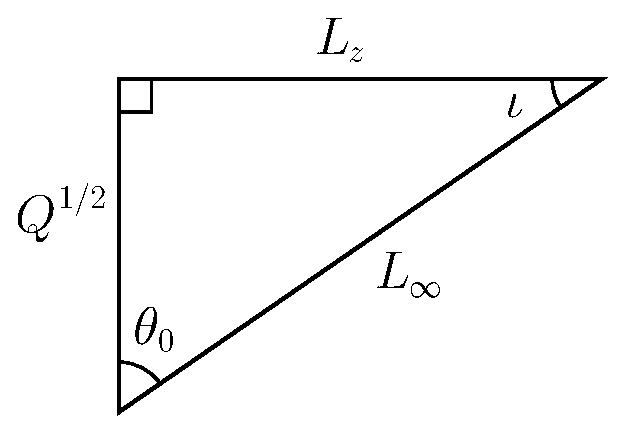
\includegraphics[width=0.35\textwidth]{./Images/Triangle.eps}
    \caption{The angular momenta $L_\infty$, $L_z$ and $\sqrt{Q}$ define a right-angled triangle. The acute angles are $\theta_0$, the extremal value of the polar angle, and $\iota$, the orbital inclination\cite{Glampedakis2002a}.}
   \label{fig:L_triangle}
\end{center}
\end{figure}
Let us now introduce a second angular variable\cite{Drasco2004}
\begin{equation}
\zeta = \zeta_0\cos^2\chi.
\end{equation}
Over one $2\pi$ period of $\chi$, $\theta$ oscillates over its full range, from its minimum value to its maximum and back. The geodesic equation for $\chi$ is
\begin{equation}
\rho^2\diff{\chi}{\tau} = \sqrt{Q + L_z^2},
\end{equation}
and may be integrated simply.

\section{Waveform Construction}

With the geodesic calculated for given angular momenta $L_z$ and $Q$, and initial starting positions, the orbiting body is assumed to follow this trajectory exactly: we ignore evolution due to the radiation of energy and angular momentum. From this we calculate the gravitational waveform using a semirelativistic approximation\cite{Ruffini1981}: we assume that the particle moves along a geodesic in the Kerr geometry, but radiates as if it were in flat spacetime. This quick-and-dirty technique is known as a numerical kludge\cite{Babak2007}.

\subsection{Kludge Approximation}

Numerical kludge approximations aim to encapsulate the main characteristics of a waveform by using the exact particle trajectory (ignoring inaccuracies from the evolution of the orbital parameters), whilst saving on computational time by using approximate waveform generation techniques. To start, we build an equivalent flat spacetime trajectory from the Kerr geodesic. This is done by identifying the Boyer-Lindquist coordinates with a set of flat-space coordinates; we consider two choices here:
\begin{enumerate}
\item Identify the Boyer-Lindquist coordinates with flat-space spherical polars \linebreak $\{r\sub{BL}, \theta\sub{BL}, \phi\sub{BL}\} \rightarrow \{r\sub{sph}, \theta\sub{sph}, \phi\sub{sph}\}$, then define flat-space Cartesian coordinates\cite{Gair2005, Babak2007}
\begin{equation}
\boldsymbol{x} = \left(r\sub{sph} \sin\theta\sub{sph}\cos\phi\sub{sph}, r\sub{sph} \sin\theta\sub{sph}\sin\phi\sub{sph}, r\sub{sph} \cos\theta\sub{sph}\right).
\end{equation}
\item Identify the Boyer-Lindquist coordinates with flat-space oblate-spheroidal coordinates $\{r\sub{BL}, \theta\sub{BL}, \phi\sub{BL}\} \rightarrow \{r\sub{ob}, \theta\sub{ob}, \phi\sub{ob}\}$ so that the flat-space Cartesian coordinates are
\begin{equation}
\boldsymbol{x} = \left(\sqrt{{r\sub{ob}}^2 + a^2} \sin\theta\sub{ob}\cos\phi\sub{ob}, \sqrt{{r\sub{ob}}^2 + a^2} \sin\theta\sub{ob}\sin\phi\sub{ob}, r\sub{ob} \cos\theta\sub{ob}\right).
\end{equation}
These are appealing because in the limit that $G \rightarrow 0$, so the gravitating mass goes to zero, the Kerr metric in Boyer-Lindquist coordinates reduces to the Minkowski metric in oblate spheroidal coordinates.%\footnote{We must take the limit $G \rightarrow 0$, rather than $M_\bullet \rightarrow 0$ to avoid the problem of an over-extreme BH with $a > M_\bullet$.}
\end{enumerate}
In the limit of $a \rightarrow 0$, the two coincide, as they do in the limit of large $r\sub{BL}$. It must be stressed that there is no well motivated argument that either coordinate system must yield an accurate GW; their use is justified {\it post facto} by comparison with results obtained from more accurate, and computationally intensive, methods\cite{Gair2005, Babak2007}. This ambiguity in assigning flat-space coordinates reflects the inconsistency of the semi-relativistic approximation: the geodesic trajectory was calculated for the Kerr geometry; by moving to flat spacetime we lose the reason for its existence. However, this inconsistency should not be regarded as a major problem; it is just an artifact of the basic assumption that the shape of the trajectory is important for determining the character of the radiation, but the curvature of the spacetime in the vicinity of the source is not. By binding the particle to the exact geodesic, we ensure that the kludge waveform has spectral components at the correct frequencies, but by assuming flat spacetime for generation of GWs they will not have the correct amplitudes.

\subsection{Quadrupole-Octopole Formula}

Now we have a flat-space particle trajectory $x\sub{p}^\mu(\tau)$, we may apply a flat-space wave generation formula. We shall use the quadrupole-octopole formula to calculate the gravitational strain\cite{Press1977, Bekenstein1973}
\begin{equation}
h^{jk}(t, \boldsymbol{x}) = -\frac{2G}{c^6r}\left[\ddot{I}^{jk} - 2n_i\ddot{S}^{ijk} + n_i\dddot{M}^{ijk}\right]_{t'\, =\, t - cr}
\label{eq:Octopole}
\end{equation}
where an over-dot represents differentiation with respect to time $t$ (and not $\tau$), $t'$ is the retarded time, $r = \left|\boldsymbol{x} - \boldsymbol{x}\sub{p}\right|$ is the radial distance, $\boldsymbol{n}$ is the radial unit vector, and the mass quadrupole ${I}^{jk}$, current quadrupole ${S}^{ijk}$ and mass octopole ${M}^{ijk}$ are defined by
\begin{align}
{I}^{jk}(t') = {} & \intd{}{}{{x'}^j{x'}^kT^{00}(t', \boldsymbol{x'})}{^3x'}\\
{S}^{ijk}(t') = {} & \intd{}{}{{x'}^j{x'}^kT^{0i}(t', \boldsymbol{x'})}{^3x'}\\
{M}^{ijk}(t') = {} & \recip{c}\intd{}{}{{x'}^i{x'}^j{x'}^kT^{00}(t', \boldsymbol{x'})}{^3x'}.
\end{align}
This is correct for a slow moving source. It is the familiar quadrupole formula\cite{Misner1973, Hobson2006}, derived from linearized theory, but with the next order term included. For a point mass the energy-momentum tensor $T^{\mu\nu}$ contains a $\delta$-function which allows easy evaluation of the integrals of the various moments to give
\begin{align}
{I}^{jk} = {} & c^2\mu x\sub{p}^jx\sub{p}^k\\
{S}^{ijk} = {} & c\mu v\sub{p}^ix\sub{p}^jx\sub{p}^k\\
{M}^{ijk} = {} & c\mu x\sub{p}^ix\sub{p}^jx\sub{p}^k.
\end{align}
To evaluate \eqnref{Octopole} we need up to the third time derivative of the position. The velocity $\boldsymbol{v}\sub{p} = \dot{\boldsymbol{x}}\sub{p}$ can be calculated from the geodesic equations: dividing by $\linediff{t}{\tau}$ gives $\dot{r}$, $\dot{\theta}$ and $\dot{\phi}$ which can then be transformed to the Cartesian velocities assuming either the spherical or oblate spheroidal coordinate system.\footnote{There is again the problem of the sign of the geodesic equations; this is simply solved by taking the sign as calculated by finite differencing the trajectory.} Expressions for the acceleration $\boldsymbol{a}\sub{p} = \ddot{\boldsymbol{x}}\sub{p}$ and the jerk $\boldsymbol{j}\sub{p} = \dddot{\boldsymbol{x}}\sub{p}$ are more involved, so these derivatives are found numerically using a simple difference formula to approximate the derivative as
\begin{equation}
\left.\diff{f}{t}\right|_{t_1} \approx \recip{2}\left[\frac{f(t_1) - f(t_0)}{t_1 - t_0} + \frac{f(t_2) - f(t_1)}{t_2 - t_1}\right],
\end{equation}
where $t_0$, $t_1$ and $t_2$ are subsequent (not necessarily uniformly spaced) time-steps.

Since we are only interested in GWs, we shall use the transverse-traceless (TT) gauge. The waveform is given in the TT gauge by\cite{Misner1973}
\begin{equation}
{h\super{TT}}_{jk} = P^l_jh_{lm}P^m_k - \recip{2}P_{jk}P^{lm}h_{lm},
\end{equation}
where the (spatial) projection operator $P_{ij}$ is
\begin{equation}
P_{ij} = \delta_{ij} - n_in_j.
\end{equation}

\section{Detection With LISA}

The LISA detector is a three-arm, space-borne laser interferometer\cite{Bender1998, Danzmann2003}. The three arms form an equilateral triangle that rotates as the system's centre of mass follows a circular, heliocentric orbit, trailing $\ang{20}$ behind the Earth. To describe the detector configuration, and to transform from the MBH coordinate system to those of the detector, we will find it useful to define three coordinate systems: those of the BH at the galactic centre $x_\bullet^i$; ecliptic coordinates centred at the solar system barycentre $x_\odot^i$, and coordinates that co-rotate with the detector $x\sub{d}^i$. The currently envisioned mission geometry is depicted in figures (??). The coordinate systems are related by a series of angles: $\Theta$ and $\Phi$ give the orientation of the solar system in the MBH's coordinates. These define the orientation of the MBH's spin axis $z_\bullet$. $\overline{\Theta}$ and $\overline{\Phi}$ give the position of the galactic centre in ecliptic coordinates. $\overline{\phi}$ gives LISA's orbital phase and $\varphi$ gives the rotational phase of the detector arms. Both of these vary linearly with time
\begin{equation}
\overline{\phi}(t) = \omega_\oplus t + \overline{\phi}_0; \quad \varphi(t) = -\omega_\oplus t + \varphi_0;
\end{equation}
where $\omega_\oplus$ corresponds to one rotation per year. Finally, $\alpha = \ang{60}$ is the inclination of the detector plane. We have computed the waveforms in the MBH's coordinates, however it is simplest to describe the measured signal using the detector's coordinates. To transform between coordinates we will use the matrix $A_{ij}$:
\begin{equation}
x\sub{d}^i = A^i_jx_\bullet^j; \quad h\sub{d}^{ij} = A^i_kA^j_lh_\bullet^{kl}.
\end{equation}
To define this, it is convenient to introduce angles
\begin{equation}
\Sigma = \overline{\Theta} + \Theta; \quad \delta = \overline{\phi} - \overline{\Phi}.
\end{equation}
The transformation matrix from the BH coordinates to the detector coordinates is
\begin{equation}
\left[A^i_j\right] = \begin{bmatrix}
a_{11} & a_{12} & a_{13} \\
a_{21} & a_{22} & a_{23} \\
a_{31} & a_{32} & a_{33}
\end{bmatrix};
\end{equation}
the elements are
\begin{align}
a_{11} = {} & s_\varphi\left(c_\delta s_\Phi - s_\delta c_\Phi c_\Sigma\right) - c_\varphi \left[s_\alpha c_\Phi s_\Sigma - c_\alpha \left(c_\delta c_\Phi c_\Sigma + s_\delta s_\Sigma\right)\right]; \\
a_{12} = {} & -s_\varphi\left(c_\delta c_\Phi - s_\delta s_\Phi c_\Sigma\right) - c_\varphi \left[s_\alpha s_\Phi s_\Sigma - c_\alpha \left(c_\delta s_\Phi c_\Sigma + s_\delta s_\Sigma\right)\right]; \\
a_{13} = {} & s_\varphi s_\delta s_\Sigma - c_\varphi\left(s_\alpha c_\Sigma + c_\alpha c_\delta s_\Sigma\right); \\
a_{21} = {} & s_\varphi\left[s_\alpha c_\Phi s_\Sigma - c_\alpha \left(c_\delta c_\Phi c_\Sigma + s_\delta s_\Sigma\right)\right] - c_\varphi \left(c_\delta s_\Phi - s_\delta c_\Phi s_\Sigma\right); \\
a_{22} = {} & s_\varphi\left[s_\alpha s_\Phi s_\Sigma - c_\alpha \left(c_\delta s_\Phi c_\Sigma + s_\delta s_\Sigma\right)\right] - c_\varphi \left(c_\delta c_\Phi - s_\delta s_\Phi s_\Sigma\right); \\
a_{23} = {} & s_\varphi\left(s_\alpha c_\Sigma + c_\alpha c_\delta s_\Sigma\right) - c_\varphi s_\delta s_\Sigma; \\
a_{31} = {} & -s_\alpha\left(c_\delta c_\Phi c_\Sigma + s_\delta s_\Phi\right) - c_\alpha c_\Phi s_\Sigma; \\
a_{32} = {} & s_\alpha\left(s_\delta c_\Phi - c_\delta s_\Phi c_\Sigma\right) - c_\alpha s_\Phi s_\Sigma; \\
a_{33} = {} & s_\alpha c_\delta s_\Sigma - c_\alpha c_\Sigma;
\end{align}
where we define $s_\vartheta \equiv \sin \vartheta$ and $c_\vartheta \equiv \cos \vartheta$.

The strains measured in the three arms can be combined such that LISA behaves as a pair of $\ang{90}$ interferometers at $\ang{45}$ to each other (with signals scaled by $\nicefrac{\sqrt{3}}{2}$)\cite{Cutler1998}. We will denote the two detectors as I and II. If we label the change in the three arms lengths caused by GWs $\delta L_1$, $\delta L_2$ and $\delta L_3$, and use $L$ for the unperturbed length, then detector I measures strain
\begin{align}
h\sub{I}(t) = {} & \frac{\delta L_1 - \delta L_2}{L} \\
 = {} & \frac{\sqrt{3}}{2}\left(\recip{2} h\sub{d}^{xx} - \recip{2}h\sub{d}^{yy}\right),
\end{align}
and detector II measures
\begin{align}
h\sub{II}(t) = {} & \frac{\delta L_1 + \delta L_2 - 2 \delta L_3}{\sqrt{3}L} \\
 = {} & \frac{\sqrt{3}}{2}\left(\recip{2} h\sub{d}^{xy} + \recip{2} h\sub{d}^{yx}\right).
\end{align}
We will use vector notation $\boldsymbol{h}(t) = \left(h\sub{I}(t), h\sub{II}(t)\right) = \left\{h_A(t)\right\}$ to represent signals from both detectors.

The final consideration for calculating the signal measured by LISA is the time of arrival of the signal: LISA's orbital position changes with time. Fortunately over the timescales of interest for parabolic encounters, these changes are small. We will assume that the position of the solar system barycentre relative to the galactic centre is constant, at least over these short timescales: it is defined by the distance $R_0$ and the angles $\overline{\Theta}$ and $\overline{\Phi}$. The time of arrival at the solar system barycentre $t_\odot$ is then the appropriate retarded time. The time of detection $t\sub{d}$ to lowest order is then
\begin{equation}
t\sub{d} \simeq t_\odot - t\sub{AU}\cos\left[\overline{\phi}(t_\odot) - \overline{\Phi}\right]\sin\overline{\Theta},
\end{equation}
where $t\sub{AU}$ is the light travel-time for LISA's orbital radius. The time $t\sub{d}$ must be used for $\phi(t)$ and $\varphi(t)$.

\section{Signal Analysis}

\subsection{Frequency Domain Formalism}

At this stage we now know the GW $\boldsymbol{h}(t)$ that will be incident upon the LISA detector. We must now discuss how to analyse the waveform to extract the information it contains. We begin with a brief overview of the basic components of signal analysis used for GWs, with application to LISA in particular. This fixes the notation we will employ. A more complete discussion of material presented here can be found in the work of Finn\cite{Finn1992}, and Cutler and Flanagan\cite{Cutler1994}.

The actual measured strain $\boldsymbol{s}(t)$ will be the combination of the signal and the detector noise
\begin{equation}
\boldsymbol{s}(t) = \boldsymbol{h}(t) + \boldsymbol{n}(t),
\end{equation}
we will assume that the noise $n_A(t)$ is stationary and Gaussian. When analysing signals, it is most convenient to work with the Fourier transform
\begin{equation}
\tilde{g}(f) = \intd{-\infty}{\infty}{g(t)e^{2\pi i ft}}{t}.
\end{equation}
Since we have assumed Gaussianity for the noise signal $n_A(t)$, each Fourier component $\tilde{n}_A(f)$ also has a Gaussian probability distribution; the assumption of stationarity means that different Fourier components are uncorrelated, thus\cite{Cutler1994}
\begin{equation}
\left\langle\tilde{n}_A(f)\tilde{n}_B^*(f')\right\rangle_n = \recip{2}\delta(f - f')S_{AB}(f),
\end{equation}
where $\left\langle\ldots\right\rangle_n$ denotes the expectation value over the noise distribution, and $S_{AB}(f)$ is the (single-sided) noise spectral density. For simplicity, we may assume that the noise in the two detectors is uncorrelated, but share the same characterization so that\cite{Cutler1998}
\begin{equation}
S_{AB}(f) = S_n(f)\delta_{AB}.
\end{equation}
The functional form of the noise spectral density $S_n(f)$ for LISA is discussed below in \secref{Noise}.

The properties of the noise allow us to define a natural inner product and associated distance on the space of signals\cite{Cutler1994}
\begin{equation}
\innerprod{\boldsymbol{g}}{\boldsymbol{k}} = 2\intd{0}{\infty}{\frac{\tilde{g}_A^*(f)\tilde{k}_A(f) + \tilde{g}_A(f)\tilde{k}_A^*(f)}{S_n(f)}}{f}.
\label{eq:inner}
\end{equation}
Using this definition, the probability of a particular realization of noise $\boldsymbol{n}(t) = \boldsymbol{n}_0(t)$ is
\begin{equation}
p(\boldsymbol{n}(t) = \boldsymbol{n}_0(t)) \propto \exp\left[-\recip{2}\innerprod{\boldsymbol{n}_0}{\boldsymbol{n}_0}\right].
\end{equation}
Thus, if the incident waveform is given as $\boldsymbol{h}(t)$, the probability of measuring signal $\boldsymbol{s}(t)$ is
\begin{equation}
p(\boldsymbol{s}(t)|\boldsymbol{h}(t)) \propto \exp\left[-\recip{2}\innerprod{\boldsymbol{s}-\boldsymbol{h}}{\boldsymbol{s}-\boldsymbol{h}}\right].
\label{eq:sig_prob}
\end{equation}

\subsection{LISA Noise Curve}\label{sec:Noise}

LISA's noise has two sources: instrumental noise and confusion noise, primarily from white dwarf binaries. The latter may be divided into contributions from galactic and extragalactic binaries. In this work we use the noise model of Barack and Cutler\cite{Barack2004}. The shape of the noise curve can be seen in \figref{Noise}. The instrumental noise dominates at both high and low frequencies. The confusion noise is important at intermediate frequencies, and is responsible for the cusp around $f = \SI{1e-3}{\Hz}$.
\begin{figure}
\begin{center}
{\resizebox{0.7\textwidth}{!}{\import{./Images/}{Noise.tex}}}
\caption{Approximate noise curve for LISA\cite{Barack2004}. The solid line includes both instrumental and confusion noise, while the dashed line shows only instrumental.}
\label{fig:Noise}
\end{center}
\end{figure}

\subsection{Window Functions}

There is one remaining complication regarding signal analysis. When we perform a Fourier transform using a computer we must necessarily only transform a finite time-span (it is a discrete Fourier transform).\footnote{The time-span in this case is the length of time the trajectory was calculated for.} The effect of this is the same as transforming the true, infinite signal multiplied by a unit top hat function of width equal to the time-span. Fourier transforming this yields the true waveform convolved with a $\sinc$. If $\tilde{h}'(f)$ is the computed Fourier transform then
\begin{align}
\tilde{h}'(f) = {} & \intd{0}{\tau}{h(t)e^{2\pi i ft}}{t} \\
 = {} & \left[\tilde{h}(f) \ast e^{-\pi if\tau}\tau \sinc(\pi f\tau)\right],
\end{align}
where $\tilde{h}(f) = \mathscr{F}\{h(t)\}$, is the unwindowed Fourier transform. This windowing of the data is an inherent problem in the method; it will be as much of a problem when analysing signals from LISA as it is computing waveforms here. Windowing causes spectral leakage, which means that a contribution from large amplitude spectral components leaks into other components (sidelobes), obscuring and distorting the spectrum at these frequencies\cite{Jones1982,Harris1978}.

\Figref{Rectangular} shows the computed Fourier transforms for an example parabolic encounter.
\begin{figure}[htbp]
  \begin{center}
   \subfigure[]{\resizebox{0.45\textwidth}{!}{\import{./Images/}{h_I_Rectangular.tex}}} \quad
   \subfigure[]{\resizebox{0.45\textwidth}{!}{\import{./Images/}{h_II_Rectangular.tex}}} \\
    \caption{Example spectra calculated using a rectangular window.  The high-frequency tail is the result of spectral leakage. The input parameters are: $M_\bullet = \num{4.3e6} M_\odot$, $a = 0.5 M_\bullet$, $\Theta = \pi/3$, $\Phi = 0$, $R_0 = \SI{8.33}{\kilo\parsec}$, $\overline{\Theta} = \ang{95.607669}$, $\overline{\Phi} = \ang{266.851760}$, $\overline{\phi}_0 = 0$, $\varphi_0 = 0$, $L_z = 10.44 M_\bullet$, $Q = 0.055 M_\bullet^2$, $\mu = 5 M_\odot$, $x_0 = \SI{3.5e12}{\metre}$, $y_0 = \SI{3.0e12}{\metre}$, $z_0 = \SI{1.0e11}{\metre}$; see \secfre{Parameters} for a discussion of these parameters. The periapse distance is $r\sub{p} = 52.7 M_\bullet$. The high-frequency tail is the result of spectral leakage. The level of the LISA noise curve is indicated by the dashed line.}
    \label{fig:Rectangular}
  \end{center}
\end{figure}
The waveforms have two distinct regions: a low-frequency curve, and a high-frequency tail. The low-frequency signal is the spectrum we are interested in; the high-frequency components are the result of spectral leakage. The $\order{\nicerecip{f}}$ behaviour of the $\sinc$ gives the shape of the tail. This has possibly been misidentified by Burko and Khanna\cite{Burko2007} as the characteristic strain for parabolic encounters.

Despite being many orders of magnitude below the peak level, the high-frequency tail is still well above the noise curve for a wide range of frequencies. It will therefore contribute to the evaluation of any inner products, and may mask interesting features. Unfortunately this is a fundamental problem that cannot be resolved completely. However, it is possible to reduce the amount of spectral leakage using apodization: to improve the frequency response of a finite time series one can use a number of weighting window functions $w(t)$ which modify the impulse response in a prescribed way. The simplest window function is the rectangular (or Dirichlet) window; this is just the top hat described above. Other window functions are generally tapered. The introduction of a window function influences the spectrum in a manner dependent upon its precise shape; there are two distinct distortions: local smearing due to the finite width of the centre lobe, and distant leakage due to finite amplitude side lobes. Choosing a window function is a trade-off between these two sources of error.

There are a wide range of window functions described in the literature\cite{Harris1978,Kaiser1980,Nuttall1981}. Since we are interested in a large dynamic range, it is necessary to pick a windowing function with an exceptionally low sidelobes. We have opted for the Nuttall 4-term window with continuous first derivative\cite{Nuttall1981}.\footnote{The Blackman-Harris minimum 4-term window\cite{Harris1978, Nuttall1981}, and the Kaiser-Bessel window\cite{Harris1978, Kaiser1980} give almost identical results.} This has low peak sidelobe and asymptotically decays away as $\nicerecip{f^3}$. \Figref{Nuttall} shows the waveform obtained using this window.
\begin{figure}[htbp]
  \begin{center}
   \subfigure[]{\resizebox{0.45\textwidth}{!}{\import{./Images/}{h_I_Nuttall_first_derivative.tex}}} \quad
   \subfigure[]{\resizebox{0.45\textwidth}{!}{\import{./Images/}{h_II_Nuttall_first_derivative.tex}}} \\
    \caption{Example spectra calculated using Nuttall's 4-term window with continuous first derivative\cite{Nuttall1981}. The input parameters are identical to those used for \figref{Rectangular}. Although this window has good sidelobe behaviour, it is still not enough to suppress spectral leakage below the LISA noise level, the dashed line, at all frequencies.}
    \label{fig:Nuttall}
  \end{center}
\end{figure}
The spectral leakage is greatly reduced.

When using a tapered window function it is important to ensure that the window is centred upon the signal; otherwise the calculated transform will have a reduced amplitude.

\section{Parameter Estimation \& Waveforms}

\subsection{Model Parameters}\label{sec:Parameters}

The shape of the waveform depends on a number of parameters: those defining the MBH; those defining the companion object on its orbits, and those defining the LISA detector. Let us define $\boldsymbol{\lambda} = \{\lambda^1, \lambda^2, \ldots, \lambda^N\}$ as the set of $N$ parameters which define the GW. For our model the input parameters for the are:
\begin{center}
\setlength{\tabcolsep}{3pt}
\begin{longtable}[0.85\textwidth]{r p{0.85\textwidth}}
1. & The MBH's mass $M_\bullet$. This is currently well constrained by the observation of stellar orbits about Sgr A*\cite{Ghez2008, Gillessen2009}, with the best estimate being $M_\bullet = (4.31 \pm 0.36) \times 10^6 M_\odot$. However this depends upon the galactic centre distance $R_0$ being accurately known. If the uncertainty in this is included $M_\bullet = (3.95 \pm 0.06|\sub{stat} \pm 0.18|_{R_0, \, \mathrm{stat}} \pm  0.31|_{R_0, \, \mathrm{sys}}) \times 10^6 M_\odot (R_0 / \SI{8}{\kilo\parsec})^{2.19}$, where the errors are statistical independent of $R_0$, statistical from the determination of $R_0$, and systematic from $R_0$.\\
2. & The spin parameter $a$. Naively we may expect this to be anywhere in the range $|a| < M_\bullet$, however the spin parameter may be limited by the accretion history. Considering the torque from radiation emitted by an accretion disc and swallowed by the BH it may be argued that $|a| \lesssim 0.998 M_\bullet$\cite{Thorne1974}. If the MBH grew via a series of randomly orientated accretion events, then the spin parameter can be low, and we would expect an average value $|a| \sim \numrange[tophrase=dash]{0.1}{0.3} M_\bullet$\cite{King2006, King2008}.\\
3. & The polar angle $\Theta$ defining the propagation direction.\\
4. & The solar system-galactic centre distance $R_0$. As for $M_\bullet$, this is constrained by stellar orbits, the best estimate is\cite{Gillessen2009} $R_0 = \SI[seperr]{8.33(35)}{\kilo\parsec}$.\\
5, 6. & The coordinates of the MBH from the solar system barycentre $\overline{\Theta}$ and $\overline{\Phi}$. These may be taken as the coordinates of Sgr A*, as the radio source is expected to be within ten Schwarzscild radii of the MBH\cite{Reid2003}. At the epoch J2000.0\cite{Reid1999} $\overline{\Theta} = \ang{95.607669}$, $\overline{\Phi} = \ang{266.851760}$. This will change with time due to the rotation of the solar system about the galactic centre, the proper motion is about $\SI{6}{\milli\as\per\yr}$, mostly in the plane of the galaxy\cite{Reid1999, Backer1999, Reid2003}.\\
7. & The angular momentum of the orbit about the MBH's spin axis $L_z$.\\
8. & The Carter's constant for the orbit $Q$.\\
9. & The mass of the orbiting particle $\mu$. This will depend upon the type of object: whether it is a MS star, WD, NS or BH.\\
10--12. & The initial position of the particle $(x_0, y_0, z_0)$. For specific values of $Q$ and $L_z$ there is a definite upper limit on $|z_0|/\sqrt{x_0^2+y_0^2}$ given by the size of $\theta_0$ from \eqnref{theta_0}.\\
13, 14. & The orbital position of the LISA satellites given by $\overline{phi}$ and $\varphi$.
\end{longtable}
\end{center}
The azimuthal angle $\Phi$ is omitted, since it arbitrarily defines the orientation of the MBH's $x$- and $y$-axes. We shall define it to be zero without loss of generality. We thus have a $14$-dimensional parameter space. However, for a given signal arrival time the orbital parameters of LISA will be known; we will not try to infer these. In lieu of anything better, we will assume fiducial initial values of zero, $\overline{\phi}_0 = 0$, $\varphi_0 = 0$.\footnote{The values of $\overline{\phi}_0$ and $\varphi_0$ do change the observed waveforms, altering the strain measured in the two arms. We do not investigate the full implications of this since we already have a large number of variables to consider, and because we will not know how $\overline{\phi}$ and $\varphi$ will be related until the mission geometry is finalised.} This leaves us with a $12$-dimensional parameter space to explore.

\subsection{Waveforms}

Figures \ref{fig:Orbit_1}--\ref{fig:Orbit_7} show example waveforms to demonstrate some of the possible variations in the signal. All these examples assume $M_\bullet = \SI{8.6e31}{\kg} \simeq \num{4.3e6} M_\odot$, $R_0 = \SI{8.33}{\kilo\parsec}$, $\overline{\Theta} = \ang{95.607669}$, $\overline{\Phi} = \ang{266.851760}$ and $\mu = \SI{1e31}{\kg} \simeq 5 M_\odot$; the other parameters are specified in the figure captions.
\begin{figure}[htbp]
  \begin{center}
   \subfigure[]{\resizebox{0.45\textwidth}{!}{\import{./Images/}{h_I_1.tex}}} \quad
   \subfigure[]{\resizebox{0.45\textwidth}{!}{\import{./Images/}{h_II_1.tex}}} \\
    \caption{Waveform for model parameters: $a = 0.5 M_\bullet$, $\Theta = \pi/3$, $L_z = 3.666 M_\bullet$, $Q = 0.409 M_\bullet^2$, , $x_0 = \SI{3.0e12}{\metre}$, $y_0 = \SI{4.0e12}{\metre}$, $z_0 = \SI{2.0e11}{\metre}$. The periapse distance is $r\sub{p} = 4.67 M_\bullet$.}
    \label{fig:Orbit_1}
  \end{center}
\end{figure}
\begin{figure}[htbp]
  \begin{center}
   \subfigure[]{\resizebox{0.45\textwidth}{!}{\import{./Images/}{h_I_2.tex}}} \quad
   \subfigure[]{\resizebox{0.45\textwidth}{!}{\import{./Images/}{h_II_2.tex}}} \\
    \caption{Waveform for model parameters: $a = 0.5 M_\bullet$, $\Theta = \pi/3$, $L_z = 5.223 M_\bullet$, $Q = 0.055 M_\bullet^2$, , $x_0 = \SI{3.5e12}{\metre}$, $y_0 = \SI{3.5e12}{\metre}$, $z_0 = \SI{1.0e11}{\metre}$. The periapse distance is $r\sub{p} = 11.77 M_\bullet$.}
    \label{fig:Orbit_2}
  \end{center}
\end{figure}
\begin{figure}[htbp]
  \begin{center}
   \subfigure[]{\resizebox{0.45\textwidth}{!}{\import{./Images/}{h_I_5.tex}}} \quad
   \subfigure[]{\resizebox{0.45\textwidth}{!}{\import{./Images/}{h_II_5.tex}}} \\
    \caption{Waveform for model parameters: $a = 0.2 M_\bullet$, $\Theta = \pi/2$, $L_z = 10.446 M_\bullet$, $Q = 2.182 M_\bullet^2$, , $x_0 = \SI{3.5e12}{\metre}$, $y_0 = \SI{3.5e12}{\metre}$, $z_0 = \SI{5.0e11}{\metre}$. The periapse distance is $r\sub{p} = 53.653 M_\bullet$.}
    \label{fig:Oribt_5}
  \end{center}
\end{figure}
\begin{figure}[htbp]
  \begin{center}
   \subfigure[]{\resizebox{0.45\textwidth}{!}{\import{./Images/}{h_I_6.tex}}} \quad
   \subfigure[]{\resizebox{0.45\textwidth}{!}{\import{./Images/}{h_II_6.tex}}} \\
    \caption{Waveform for model parameters: $a = 0.7 M_\bullet$, $\Theta = \pi/2$, $L_z = 5.223 M_\bullet$, $Q = 21.824 M_\bullet^2$, , $x_0 = \SI{2.8e12}{\metre}$, $y_0 = \SI{2.8e12}{\metre}$, $z_0 = \SI{3.0e12}{\metre}$. The periapse distance is $r\sub{p} = 22.699 M_\bullet$.}
    \label{fig:Orbit_6}
  \end{center}
\end{figure}
\begin{figure}[htbp]
  \begin{center}
   \subfigure[]{\resizebox{0.45\textwidth}{!}{\import{./Images/}{h_I_7.tex}}} \quad
   \subfigure[]{\resizebox{0.45\textwidth}{!}{\import{./Images/}{h_II_7.tex}}} \\
    \caption{Waveform for model parameters: $a = 0.7 M_\bullet$, $\Theta = \pi/2$, $L_z = 15.669 M_\bullet$, $Q = 84.559 M_\bullet^2$, , $x_0 = \SI{1.0e12}{\metre}$, $y_0 = \SI{4.2e12}{\metre}$, $z_0 = \SI{1.0e12}{\metre}$. The periapse distance is $r\sub{p} = 148.157 M_\bullet$.}
    \label{fig:Orbit_7}
  \end{center}
\end{figure}

\subsection{Inference \& Fisher Matrices}

Having detected a GW signal $\boldsymbol{s}(t)$ we are interested in what we may learn about the source. We have an inference problem that may be solved by appropriate application of Bayes' Theorem\cite{Jaynes2003}: the probability distribution for our parameters given that we have detected the signal $\boldsymbol{s}(t)$ is given by the posterior
\begin{equation}
p(\boldsymbol{\lambda}|\boldsymbol{s}(t)) = \frac{p(\boldsymbol{s}(t)|\boldsymbol{\lambda})p(\boldsymbol{\lambda})}{p(\boldsymbol{s}(t))}.
\end{equation}
Here $p(\boldsymbol{s}(t)|\boldsymbol{\lambda})$ is the likelihood of the parameters, $p(\boldsymbol{\lambda})$ is the prior probability distribution for the parameters, and $p(\boldsymbol{s}(t)) = \intd{}{}{p(\boldsymbol{s}(t)|\boldsymbol{\lambda})}{^N \lambda}$ is, for our purposes, a normalising constant and may be ignored. The likelihood function depends upon the particular realization of noise. A particular set of parameters $\boldsymbol{\lambda}_0$ defines a waveform $\boldsymbol{h}_0(t) = \boldsymbol{h}(t; \boldsymbol{\lambda}_0)$, the probability that we observe signal $\boldsymbol{s}(t)$ for this GW is given by \eqnref{sig_prob}, so the likelihood is just
\begin{equation}
p(\boldsymbol{s}(t)|\boldsymbol{\lambda}_0) \propto \exp\left[-\recip{2}\innerprod{\boldsymbol{s}-\boldsymbol{h}_0}{\boldsymbol{s}-\boldsymbol{h}_0}\right].
\end{equation}
If we were to define this as a probability distribution for the parameters $\boldsymbol{\lambda}$, then the modal values would be the maximum-likelihood parameters $\boldsymbol{\lambda}\sub{ML}$. The waveform $h(t; \boldsymbol{\lambda}\sub{ML})$ would be the signal closest to $\boldsymbol{s}(t)$ in the space of all signals, where distance is defined using the inner product \eqnref{inner}\cite{Cutler1994}.

In the limit of a high signal-to-noise ratio (SNR), we may approximate this as\cite{Vallisneri2008}
\begin{equation}
p(\boldsymbol{s}(t)|\boldsymbol{\lambda}_0) \propto \exp\left[-\recip{2}\innerprod{\partial_a\boldsymbol{h}}{\partial_b\boldsymbol{h}}\left(\lambda^a - \langle\lambda^a\rangle_\ell\right)\left(\lambda^b - \langle\lambda^b\rangle_\ell\right)\right],
\end{equation}
where the mean is defined as
\begin{equation}
\langle\lambda^a\rangle_\ell = \frac{\intd{}{}{\lambda^a p(\boldsymbol{s}(t)|\boldsymbol{\lambda})}{^N \lambda}}{\intd{}{}{p(\boldsymbol{s}(t)|\boldsymbol{\lambda})}{^N \lambda}}.
\end{equation}
Using the high SNR limit approximation, this mean is just the maximum-likelihood value $\langle\lambda^a\rangle_\ell = \lambda^a\sub{ML}$. The quantity
\begin{equation}
\Gamma_{ab} = \innerprod{\partial_a\boldsymbol{h}}{\partial_b\boldsymbol{h}}
\end{equation}
is the Fisher information matrix. We see that it controls the variance of the likelihood distribution.

The form of the posterior distribution will depend upon the nature of the prior information. If we have an uninformative prior, such that $p(\boldsymbol{\lambda})$ is a constant, then the posterior distribution would be determined by the likelihood. In the high SNR limit, we would obtain a Gaussian with variance-covariance matrix
\begin{equation}
\boldsymbol{\Sigma} = \boldsymbol{\Gamma}^{-1}.
\end{equation}
The Fisher information matrix gives the uncertainty associated with the estimated parameter values, in this case the maximum-likelihood values. If the prior were to restrict the allowed range of parameters, for example, as we do for the spin parameter is $|a|$; then the posterior would be a truncated Gaussian, and $\boldsymbol{\Gamma}^{-1}$ would no longer represent the variance-covariance. If the prior was approximately Gaussian with variance-covariance matrix $\boldsymbol{\Sigma}_0$, then the posterior would also be Gaussian.\footnote{If we only know the typical value and spread of a parameter then a Gaussian is the maximum entropy prior\cite{Jaynes2003}: the prior that is least informative given what we do know, the prior that best reflects our state of ignorance.} The posterior variance-covariance would be\cite{Cutler1994, Vallisneri2008}
\begin{equation}
\boldsymbol{\Sigma} = \left(\boldsymbol{\Gamma} + \boldsymbol{\Sigma}_0^{-1}\right)^{-1}.
\end{equation}
From this the inverse Fisher matrix $\boldsymbol{\Gamma}^{-1}$ is a lower bound on the size of the covariance matrix.\footnote{It may also be shown to be the Cram\'{e}r-Rao bound on the error covariance of an unbiased estimator\cite{Cutler1994, Vallisneri2008}. Thus it represents the frequentist error: the lower bound on the covariance for an unbiased parameter estimator $\boldsymbol{\lambda}\sub{est}$ calculated from an infinite set of experiments with the same signal $\boldsymbol{h}(t)$ but different realizations of the noise $\boldsymbol{n}(t)$.}

As a first estimate of what we may learn from parabolic encounters we have only looked at the Fisher information matrix elements. If these are large then we expect we would be able to precisely determine a parameter, whereas if they are small we would not be able to learn much more than we already believe from our prior knowledge.

\subsection{Inverse Fisher Matrices}

Calculating the inverse Fisher matrix for example orbits, we find that there is a large degeneracy between the mass $\mu$ and the distance $R_0$. This is not surprising since primarily role of both is determining the amplitude of the waveform in \eqnref{Octopole}. This is the only place that $\mu$ appears. We will not be able to determine both from an EMRB. Unless we can determine the mass of the object by other means, which seems unlikely, it appears that we must give up on determining $R_0$. Instead we should accept our prior value and remove $R_0$ from our parameter set. The inverse Fisher matrix's elements for some example orbits are tabulated in the appendix. For the values presented here the parameters are normalised with respect to their maximum likelihood values $\widehat{\lambda}^a = \lambda^a/\lambda\sub{ML}^a$; the Fisher matrices are calculated by differentiating with respect to these parameters so that $\boldsymbol{\Gamma}^{-1}$ gives the relative variance-covariance.

\section{Energy Spectra}

To check that the NK waveforms are sensible, we may compare the energy spectra calculated from these waveform with those obtained from the classic treatment of Peters and Matthews\cite{Peters1963, Peters1964}. This calculates GW emission for Keplerian orbits in flat spacetime, assuming only quadrupole radiation. The spectrum produced should be similar to that obtained from the NK in weak fields, that is for orbits with a large periapsis; however we do not expect an exact match because of the differing input physics and various approximations.  We do not intend to use the kludge waveforms to calculate an accurate energy flux: this would be inconsistent as we assume that the orbits do not evolve with time. We only calculate the energy flux as a sanity check; to check that the kludge approximation is consistent with other approaches.

\subsection{Kludge Spectrum}

Our gravitational wave in the TT gauge has momentum pseudotensor\cite{Misner1973}
\begin{equation}
T_{\mu\nu} = \frac{c^4}{32\pi G}\left\langle\partial_\mu h_{ij} \partial_\nu h^{ij}\right\rangle,
\end{equation}
where $\langle\ldots\rangle$ indicates averaging over several wavelengths, or equivalently averaging over several periods. Thus, the flux of energy through a sphere of radius $r = R$ is
\begin{equation}
\diff{E}{t} = \frac{c^3}{32\pi G} R^2 \int{\dd\Omega}\left\langle\diff{h_{ij}}{t}\diff{h^{ij}}{t}\right\rangle,
\end{equation}
with $\int{\dd\Omega}$ representing integration over all solid angles. From \eqnref{Octopole} we see that the waves have a $\nicerecip{r}$ dependence, so if we define
\begin{equation}
h_{ij} = \frac{H_{ij}}{r},
\end{equation}
we see that the flux is independent of $R$, as required for energy conservation,
\begin{equation}
\diff{E}{t} = \frac{c^3}{32\pi G} \int{\dd\Omega}\left\langle\diff{H_{ij}}{t}\diff{H^{ij}}{t}\right\rangle.
\end{equation}
If we now integrate to find the total energy emitted we obtain
\begin{equation}
E = \frac{c^3}{32\pi G} \int{\dd\Omega}\int_{-\infty}^{\infty}{\dd t} \, \diff{H_{ij}}{t}\diff{H^{ij}}{t}.
\end{equation}
Since we are considering all time, the localization of the energy is no longer of importance and so it is unnecessary to average over several periods. If we switch to Fourier representation $\widetilde{H}_{ij}(f) = \mathscr{F}\{H_{ij}(t)\}$, then
\begin{align}
E = {} & \frac{c^3}{32\pi G} \int{\dd\Omega}\int_{-\infty}^{\infty}{\dd t}\intd{-\infty}{\infty}{}{f} \, 2\pi i f \widetilde{H}_{ij}(f)e^{2\pi i f t}\int_{-\infty}^{\infty}{\dd f'} \, 2\pi i f' \widetilde{H}^{ij}(f')e^{2\pi i f' t} \nonumber \\
 = {} & \frac{\pi c^3}{8 G} \int{\dd\Omega}\int_{-\infty}^{\infty}{\dd f} \, f^2 \widetilde{H}_{ij}(f)\widetilde{H}^{ij}(-f) \nonumber \\
 = {} & \frac{\pi c^3}{4 G} \int{\dd\Omega}\int_{0}^{\infty}{\dd f} \, f^2 \widetilde{H}^{ij}(f)\widetilde{H}_{ij}^*(f).
\end{align}
Here we have used the fact that the signal is real so that $\widetilde{H}_{ij}^*(f) = \widetilde{H}_{ij}(-f)$. Using this we can identify the energy spectrum as
\begin{align}
\diff{E}{f} = \frac{\pi c^3}{4 G} \intd{}{}{}{\Omega} \, f^2 \widetilde{H}^{ij}(f)\widetilde{H}_{ij}^*(f).
\label{eq:NK_dEdf}
\end{align}

\subsection{Peters \& Matthews Spectrum}

To calculate the energy spectrum for a parabolic orbit, we follow the derivation of Gair\cite{Gair2010}. Peters and Matthews give the power radiated into the $n$th harmonic of the orbital angular frequency as
\begin{equation}
P(n) = \frac{32}{5}\frac{G^4}{c^5}\frac{M_\bullet^2\mu^2(M_\bullet + \mu)(1-e)^5}{{r\sub{p}}^5}g(n,e)
\label{eq:PM_P}
\end{equation}
where the function $g(n,e)$ is defined in terms of Bessel functions of the first kind
\begin{align}
g(n,e) = {} & \frac{n^4}{32}\left\{\left[J_{n-2}(ne) - 2eJ_{n-1}(ne) + \frac{2}{n}J_n(ne) + 2eJ_{n+1}(ne) - J_{n+2}(ne)\right]^2 \right. \nonumber \\
 & + \left. \left(1 - e^2\right)\left[J_{n-2}(ne) - 2J_n(ne) + J_{n+2}(ne)\right]^2 + \frac{4}{3n^2}\left[J_n(ne)\right]^2\right\}.
\end{align}
The Keplerian orbital frequency is
\begin{align}
{\omega_0}^2 = {} & \frac{G(M_\bullet + \mu)(1-e)^3}{{r\sub{p}}^3}\\
 = {} & (1-e)^3{\omega\sub{c}}^2,
\label{eq:Kepler_freq}
\end{align}
where $\omega\sub{c}$ is defined as the orbital angular frequency of a circular orbit of radius equal to $r\sub{p}$. The total energy radiated into the $n$th harmonic, that is at frequency $\omega_n = n\omega_0$, is the power multiplied by the orbital period
\begin{equation}
E(n) = \frac{2\pi}{\omega_0}P(n);
\label{eq:E(n)}
\end{equation}
as $e \rightarrow 1$ for a parabolic orbit, $\omega_0 \rightarrow 0$ so the orbital period becomes infinite. We may therefore identify the energy radiated per orbit with the total orbital energy radiated. Since the spacing of harmonics is $\Delta\omega = \omega_0$, we may identify the energy spectrum
\begin{equation}
\left.\diff{E}{\omega}\right|_{\omega_n}\omega_0 = E(n).
\end{equation}
Using the above relations, and changing to linear frequency $2\pi f = \omega$, we obtain
\begin{align}
\left.\diff{E}{f}\right|_{f_n} = {} & \frac{128\pi^2}{5}\frac{G^3}{c^5}\frac{M_\bullet^2\mu^2}{r\sub{p}^2}(1-e)^2g(n,e) \\
 = {} & \frac{4\pi^2}{5}\frac{G^3}{c^5}\frac{M_\bullet^2\mu^2}{r\sub{p}^2}\ell(n,e),
\label{eq:PM_spectrum}
\end{align}
where we have defined the function $\ell(n,e)$ in the last line. For a parabolic orbit, we now have to take the limit of $\ell(n,e)$ as $e \rightarrow 1$. For this we shall use a number of properties of Bessel functions, and will make frequent reference to Watson\cite{Watson1995}.

We shall simplify $\ell(n,e)$ using the recurrence formulae (Watson\cite{Watson1995} 2.12)
\begin{align}
J_{\nu-1}(z) + J_{\nu+1}(z) = {} & \frac{2\nu}{z}J_\nu(z)\\
J_{\nu-1}(z) - J_{\nu+1}(z) = {} & 2J'_\nu(z).
\end{align}
We shall also eliminate $n$ using
\begin{align}
n = {} & \frac{\omega_n}{\omega_0} \nonumber \\
= {} & (1-e)^{-3/2}\widetilde{f}.
\end{align}
where $\widetilde{f} = \omega_n/\omega\sub{c} = f_n/f\sub{c}$ is a dimensionless frequency. We begin by breaking $\ell$ into three parts
\begin{align}
\ell = {} & \underbrace{(1-e)^2n^4\left[J_{n-2} - 2eJ_{n-1} + \frac{2}{n}J_n + 2eJ_{n+1} - J_{n+2}\right]^2}_{\ell_1} \nonumber \\
  & + \underbrace{(1-e)^3(1+e)n^4\left[J_{n-2} - 2J_n + J_{n+2}\right]^2}_{\ell_2} + \underbrace{\frac{4(1-e)^2n^2}{3}\left[J_n\right]^2}_{\ell_3}.
\end{align}
We have suppressed the argument of the Bessel functions for brevity. Tackling each term of $\ell$ in turn we obtain
\begin{align}
\ell_1(\widetilde{f},e) = {} & \left[\frac{4(1+e)\widetilde{f}^2}{e}\frac{J'_n}{1-e} + 2\frac{e-2}{e}\widetilde{f}\frac{J_n}{(1-e)^{1/2}}\right]^2\\
\ell_2(\widetilde{f},e) = {} & 16(1+e)\left[\frac{(1+e)\widetilde{f}^2}{e^2}\frac{J_n}{(1-e)^{1/2}} - \widetilde{f}\frac{J'_n}{e}\right]^2\\
\ell_3(\widetilde{f},e) = {} & \frac{4\widetilde{f}^2}{3}\left[{J_n}{(1-e)^{1/2}}\right]^2.
\end{align}
To take the limit of these we need to find the limiting behaviour of Bessel functions. We shall define two new functions
\begin{equation}
A(\widetilde{f}) = \lim_{e\rightarrow 1}\left\{\frac{J_n}{(1-e)^{1/2}}\right\}; \quad B(\widetilde{f}) = \lim_{e\rightarrow 1}\left\{\frac{J'_n}{1-e}\right\}.
\end{equation}
To give a well defined energy spectrum, both of these must be finite. In this case we see that the second term in $\ell_2$ should go to zero.

The Bessel function has an integral representation
\begin{equation}
J_\nu(z) = \recip{\pi}\intd{0}{\pi}{\cos(\nu\theta - z\sin\theta)}{\theta},
\end{equation}
we want the limit of this for $\nu \rightarrow \infty$, $z \rightarrow \infty$, with $z \leq \nu$. We will use the stationary phase approximation to argue that the predominant contribution to the integral comes from when the argument of the cosine is approximately zero, that is for small $\theta$ (Watson\cite{Watson1995} 8.2, 8.43). In this case we have
\begin{align}
J_\nu(z) \sim {} & \recip{\pi}\intd{0}{\pi}{\cos\left(\nu\theta - z\theta + \frac{z}{6}\theta^3\right)}{\theta}\\
 \sim {} & \recip{\pi}\intd{0}{\infty}{\cos\left(\nu\theta - z\theta + \frac{z}{6}\theta^3\right)}{\theta};
\end{align}
this last expression is an Airy integral. The Airy integral has a standard form (Watson\cite{Watson1995} 6.4)
\begin{equation}
\intd{0}{\infty}{\cos(t^3 + xt)}{t} = \frac{\sqrt{x}}{3}K_{1/3}\left(\frac{2x^{3/2}}{3^{3/2}}\right),
\end{equation}
where $K_\nu(z)$ is a modified Bessel function of the second kind. Using this to evaluate our limit gives
\begin{equation}
J_\nu(z) \sim \recip{\pi}\sqrt{\frac{2(\nu - z)}{3z}}K_{1/3}\left(\frac{2^{3/2}}{3}\sqrt{\frac{(\nu -z)^3}{z}}\right).
\end{equation}
For our particular case we have
\begin{equation}
\nu = (1 - e)^{-3/2}\widetilde{f}; \quad z = (1 - e)^{-3/2}e\widetilde{f};
\end{equation}
\begin{equation}
\frac{\nu - z}{z} = (1 - e); \quad \frac{(\nu - z)^3}{z} = \widetilde{f}^2;
\end{equation}
so we find
\begin{equation}
J_n(ne) \sim \recip{\pi}\sqrt{\frac{2}{3}}(1-e)^{1/2}K_{1/3}\left(\frac{2^{3/2}\widetilde{f}}{3}\right),
\end{equation}
thus
\begin{equation}
A(\widetilde{f}) = \recip{\pi}\sqrt{\frac{2}{3}}K_{1/3}\left(\frac{2^{3/2}\widetilde{f}}{3}\right)
\end{equation}
is well defined.

Now finding the derivative
\begin{align}
J'_\nu(z) = {} & \recip{2}\left[J_{\nu-1}(z) - J_{\nu+1}(z)\right] \nonumber \\
 \sim {} & \recip{2\pi}\left[\sqrt{\frac{2(\nu -1 - z)}{3z}}K_{1/3}\left(\frac{2^{3/2}}{3}\sqrt{\frac{(\nu - 1 - z)^3}{z}}\right) \right. \nonumber \\
  & \left. - \sqrt{\frac{2(\nu +1 - z)}{3z}}K_{1/3}\left(\frac{2^{3/2}}{3}\sqrt{\frac{(\nu + 1 - z)^3}{z}}\right)\right].
\end{align}
For our case
\begin{align}
\sqrt{\frac{\nu \pm 1 - z}{z}} = {} & (1 - e)^{1/2}\left[1 \pm \frac{(1-e)^{1/2}}{2\widetilde{f}} + \ldots\right];\\
\sqrt{\frac{(\nu \pm 1 - z)^{3/2}}{z}} = {} & \widetilde{f}\left[1 \pm \frac{3(1-e)^{1/2}}{2\widetilde{f}} + \ldots\right];
\end{align}
and so
\begin{align}
J'_n(ne) \sim {} & \recip{2\pi}\sqrt{\frac{2}{3}}(1-e)^{1/2}\left\{\left[1 - \frac{(1-e)^{1/2}}{2\widetilde{f}}\right]K_{1/3}\left(\frac{2^{3/2}\widetilde{f}}{3}\left[1 - \frac{3(1-e)^{1/2}}{2\widetilde{f}}\right]\right) \right. \nonumber \\
 & \left. - \left[1 + \frac{(1-e)^{1/2}}{2\widetilde{f}}\right]K_{1/3}\left(\frac{2^{3/2}\widetilde{f}}{3}\left[1 - \frac{3(1-e)^{1/2}}{2\widetilde{f}}\right]\right)\right]\nonumber \\
 \sim {} & \frac{-1}{2\pi}\sqrt{\frac{2}{3}}(1-e)\left[2^{3/2}K'_{1/3}\left(\frac{2^{3/2}\widetilde{f}}{3}\right) + \recip{\widetilde{f}}K_{1/3}\left(\frac{2^{3/2}\widetilde{f}}{3}\right)\right].
\end{align}
We may re-express the derivative using the recurrence formula (Watson\cite{Watson1995} 3.71)
\begin{equation}
K_{\nu-1}(z) - K_{\nu+1}(z) = -2K'_\nu(z)
\end{equation}
to give
\begin{equation}
J'_n(ne) \sim \frac{1-e}{\sqrt{3}\pi}\left[K_{-2/3}\left(\frac{2^{3/2}\widetilde{f}}{3}\right) + K_{4/3}\left(\frac{2^{3/2}\widetilde{f}}{3}\right) - \recip{\sqrt{2}\widetilde{f}}K_{1/3}\left(\frac{2^{3/2}\widetilde{f}}{3}\right)\right].
\end{equation}
And so finally,
\begin{equation}
B(\widetilde{f}) = \recip{\sqrt{3}\pi}\left[K_{-2/3}\left(\frac{2^{3/2}\widetilde{f}}{3}\right) + K_{4/3}\left(\frac{2^{3/2}\widetilde{f}}{3}\right) - \recip{\sqrt{2}\widetilde{f}}K_{1/3}\left(\frac{2^{3/2}\widetilde{f}}{3}\right)\right],
\end{equation}
which is also well defined.

Having obtained expressions for $A(\widetilde{f})$ and $B(\widetilde{f})$ in terms of standard functions, we may now calculate the energy spectrum for a parabolic orbit. From \eqnref{PM_spectrum} we have
\begin{equation}
\diff{E}{f} = \frac{4\pi^2}{5}\frac{G^3}{c^5}\frac{M_\bullet^2\mu^2}{r\sub{p}^2}\ell\left(\frac{f}{f\sub{c}}\right),
\label{eq:PM_dEdf}
\end{equation}
where we have used the limit
\begin{align}
\ell(\widetilde{f}) = {} & \lim_{e \rightarrow 1}\left\{\ell(n,e)\right\} \nonumber \\
 = {} & \left[8\widetilde{f}B(\widetilde{f}) - 2\widetilde{f}A(\widetilde{f})\right]^2 + \left(128\widetilde{f}^4 + \frac{4\widetilde{f}^2}{3}\right)\left[A(\widetilde{f})\right]^2.
\end{align}

To check the validity of this limit we may calculate the total energy radiated. We should be able to calculate this by integrating \eqnref{PM_dEdf} over all frequencies, or alternatively by summing the energy radiated into each harmonic. For consistency, the two approaches should yield the same result. First, summing over harmonics we obtain
\begin{align}
E\sub{sum} = {} & \sum_n E(n) \nonumber \\
 = {} & \frac{64\pi}{5}\frac{G^3}{c^5}\frac{M_\bullet^2\mu^2}{r\sub{p}^2}\omega\sub{c}(1-e)^{7/2}\sum_n g(n,e),
\end{align}
where we have used equations \eqref{eq:PM_P}, \eqref{eq:Kepler_freq} and \eqref{eq:E(n)}. Peters and Matthews\cite{Peters1963} provide the result
\begin{equation}
\sum_n g(n,e) = \frac{1 + \nicefrac{73}{24}\, e^2 + \nicefrac{37}{96}\, e^4}{(1-e^2)^{7/2}}.
\end{equation}
Using this,
\begin{equation}
E\sub{sum} = \frac{64\pi}{5}\frac{G^3}{c^5}\frac{M_\bullet^2\mu^2}{r\sub{p}^2}\omega\sub{c}\frac{1 + \nicefrac{73}{24}\, e^2 + \nicefrac{37}{96}\, e^4}{(1+e^2)^{7/2}}.
\end{equation}
This is perfectly well behaved as $e \rightarrow 1$. Taking the limit for a parabolic orbit, the total energy radiated is
\begin{equation}
E\sub{sum} = \frac{85\pi}{2^{5/2}3}\frac{G^3}{c^5}\frac{M_\bullet^2\mu^2}{r\sub{p}^2}\omega\sub{c}.
\end{equation}
Integrating over the energy spectrum, \eqnref{PM_dEdf}, gives
\begin{align}
E\sub{int} = {} & \intd{0}{\infty}{\diff{E}{f}}{f} \nonumber \\
 = {} & \frac{2\pi}{5}\frac{G^3}{c^5}\frac{M_\bullet^2\mu^2}{r\sub{p}^2}\omega\sub{c}\intd{0}{\infty}{\ell(\widetilde{f})}{\widetilde{f}}.
\end{align}
The integral can be easily evaluated numerically showing
\begin{align}
\intd{0}{\infty}{\ell(\widetilde{f})}{\widetilde{f}} = {} & 12.5216858\ldots \nonumber \\
 = {} & \frac{425}{2^{7/2}3},
\end{align}
and so we find that the two total energies are consistent
\begin{align}
\label{eq:PM_total}
E\sub{int} = {} & \frac{85\pi}{2^{5/2}3}\frac{G^3}{c^5}\frac{M_\bullet^2\mu^2}{r\sub{p}^2}\omega\sub{c} \\
 = {} & E\sub{sum}.
\end{align}

\subsection{Comparison}

Two energy spectra are plotted in \figref{Energy} for orbits with a periapsis of $r\sub{p} = 35.0 r\sub{S}$, where $r\sub{S}$ is the MBH's Schwarzschild radius. For consistency with the approximation of Peters and Matthews the NK waveform has been calculated using only the quadrupole formula.
\begin{figure}[htbp]
  \begin{center}
   \subfigure[]{\resizebox{0.7\textwidth}{!}{\import{./Images/}{loglog_E.tex}}} \\
   \subfigure[]{\resizebox{0.7\textwidth}{!}{\import{./Images/}{loglin_E.tex}}}
    \caption{Energy spectra for a parabolic orbit of a $\mu = \SI{1e31}{\kg} \simeq 5 M_\odot$ object about a $M_\bullet = \SI{8.6e36}{\kg} \simeq \num{4.3e6} M_\odot$ Schwarzschild MBH with $L_z = 12 M_\bullet$ and $Q = 0$; the periapse distance is $r\sub{p} = 69.9 M_\bullet$. The spectra calculated from a the NK waveform is shown by the solid line and the Peters and Matthews flux is indicated by the dashed line. The NK waveform only uses the quadrupole formula.}
    \label{fig:Energy}
  \end{center}
\end{figure}
The two spectra appear to be in good agreement, showing the same general shape. The NK spectrum is more tightly peaked, but is always within a factor of $2$ (ignoring the high-frequency tail).

We may also compare the total energy flux. The Peters and Matthews flux may be calculated from \eqnref{PM_total}. The NK flux can be found by integrating \eqnref{NK_dEdf}; it can also be found from the standard expression for GW luminosity assuming the quadrupole formula
\begin{equation}
\diff{E}{t} = \frac{G}{5c^9}\left\langle\dddot{\Ibar}_{ij}\dddot{\Ibar}^{ij}\right\rangle,
\end{equation}
where $\dddot{\Ibar}^{ij}$ is the reduced quadrupole moment. Integrating this over time gives
\begin{equation}
E = \frac{G}{5c^9}\int \dd t \dddot{\Ibar}_{ij}\dddot{\Ibar}^{ij}.
\end{equation}
Evaluating this should be more accurate than relying upon integrating \eqnref{NK_dEdf} since it is not necessary to Fourier transform, use window functions or integrate over all solid angles. For the orbit shown in \figref{Energy} integrating the NK spectrum gives $E_{\widetilde{H}(f)} = \SI{5.936e36}{\joule}$ and using the quadrupolar formula gives $E_\Ibar = \SI{5.945e36}{\joule}$. The two are consistent to $\SI{1.5}{\percent}$. The largest source of error may be from the use of the the window function, especially if it is not perfectly centred; however, the integration over all angles will also contribute since it may introduce an error of the order of a percent. From the level of this agrrement we may infer that the numerical error made in calculating $\widetilde{H}_{ij}$ is less than a percent, which should be adequate for our purposes. The Peters and Matthews total energy is $E\sub{PM} = \SI{5.747e36}{\joule}$. The total energy flux from the kludge waveform is larger than the Peters and Matthews result. This behaviour has been seen before for high eccentricity orbits about a non-spinning BH\cite{Gair2005}. From the level of agreement we may be confident that the NK waveforms are a reasonable approximation.

Introducing the octopole moments makes a small change to the energy spectrum, as seen in \figref{Energy_oct}.
\begin{figure}[htbp]
  \begin{center}
   \subfigure[]{\resizebox{0.7\textwidth}{!}{\import{./Images/}{loglog_E_oct.tex}}} \\
   \subfigure[]{\resizebox{0.7\textwidth}{!}{\import{./Images/}{loglin_E_oct.tex}}}
    \caption{Energy spectra for the same orbit as shown in \figref{Energy}. The spectra calculated from a the NK waveform is shown by the solid line and the Peters and Matthews flux is indicated by the dashed line. The NK waveform includes contributions from the current quadrupole and mass octople as given by \eqnref{Octopole}.}
    \label{fig:Energy_oct}
  \end{center}
\end{figure}
The peak of the spectrum is shifted to a slightly higher frequency, and the total energy radiated is increased to $E_{\widetilde{H}(f)} = \SI{6.202e36}{\joule}$. At such radii the higher order terms only make a correction of the order of a few percent.

\section{Discussion \& Further Work}




\chapter{Future Work}

The work outlined in previous chapters should be largely completed by the end of 2010. It may be that further investigation reveals addition avenues to explore; however, it will be necessary to find new projects as well. Development of new areas of study will depend upon what is presented in the literature in the intervening time. Current ideas are discussed below.

\section{Other Theories Of Gravity}

Analysis similar to that discussed in chapter 1 for metric $f(R)$ gravity may be performed for other theories of modified gravity. This is a rapidly developing area incorporating ideas from quantum gravity and cosmology. Other theories to be investigated could include:
\begin{itemize}
\item Metric-affine gravity\cite{Sotiriou2007, Sotiriou2007b}, as discussed in \secref{Action}. Since this is not a metric theory of gravity it may be possible to find observational tests that strongly constrain, or rule out this theory\cite{Will2006}.
\item{} Generalised higher-order gravities which replace $R$ in the Einstein-Hilbert action with $f(R, R_{\mu\nu}R^{\mu\nu}, R_{\mu\nu\rho\sigma}R^{\mu\nu\rho\sigma})$\cite{Farhoudi2006, Madsen1989}. We see that $f(R)$ is just a simplification of this case. Again we should recover the results of quadratic gravity in linearized theory\cite{Pechlaner1966, Stelle1978, Schmidt1986, Teyssandier1990, Capozziello2009b}.
\item{} Ho\v{r}ava-Lifshitz gravity\cite{Horava2009, Blas2010a, Sotiriou2009c} which sacrifices spacetime covariance in favour of being renormalizable. A preferred foliation of space and time along the lines of the Arnowitt-Deser-Misner (ADM) formalism is adopted\cite{Arnowitt1962a}, with Lorentz invariance being emergent at large distances. This removes many of the problems associated with time traditionally associated with trying to quantize GR.
\item{} Chern-Simons modified gravity\cite{Alexander2009a} which includes gravitational parity violation. Motivated by gauge theories, Chern-Simons gravity includes a term in the action proportional to the Pontryagin density ${^\ast R} R = \nicerecip{2}\epsilon^{\nu\rho\sigma\tau}{R^\lambda}_{\mu\sigma\tau}{R^\mu}_{\lambda\nu\rho}$, where $\epsilon^{\nu\rho\sigma\tau}$ is the Levi-Civita alternating tensor, coupled to a (pseudo-)scalar filed $\vartheta$. Consequences of this include birefringent gravitational waves, altered precession rates, and the modification of vacuum solutions that are axisymmetric but not spherically symmetric such as Kerr.
\end{itemize}
Since there are so many ways to formulate an alternate theory of gravity, there are many opportunities for study in this area. It would be desirable to find tests that can distinguish these theories from each other and GR; strong-field tests seem the most promising.

\section{Observing Black Hole Shadows}

Black holes are intriguing objects. In the next few years it is hoped that VLBI will advance to the stage that it will be possible to resolve features of the size of the order of the event horizon\cite{Doeleman2008}. This capability would allow us to directly image accretion flows down to the event horizon, and would be the first direct evidence that these compact objects are actually black holes as currently understood, not some other exotic compact object.

One of the main targets of these strong-field VLBI observations is the measurement of the BH's shadow. This is the dark region surrounding the BH from which no light can reach the observer; it is bounded by the innermost photon orbit\cite{Chandrasekhar1998}. The exact shape of the shadow is intimately linked to the metric and is a sensitive probe of the spacetime. By measuring the shape of the shadow it may be possible to measure the spin and inclination of the BH\cite{Hioki2009a}, assuming it is Kerr, check whether it is an over-extreme Kerr black hole\cite{Bambi2009}, or even probe deviations from Kerr\cite{Johannsen2010a, Johannsen2010b}. It would be interesting to investigate the shape of the shadow in other spacetimes, for example Manko-Novikov\cite{Manko1992, Gair2008a} which form a family of exact asymptotically flat spacetimes with arbitrary multipole moments. The shape of the shadow of a Kerr BH is shown in \figref{Shadow}.
\begin{figure}[htb]
  \begin{center}
   \subfigure[$a = -0.2 M_\bullet$, $\theta\sub{obs} = \pi/2$]{\resizebox{0.3\textwidth}{!}{\import{./Images/}{Shadow_2-psfrag.tex}}} \quad
   \subfigure[$a = -0.2 M_\bullet$, $\theta\sub{obs} = \pi/6$]{\resizebox{0.3\textwidth}{!}{\import{./Images/}{Shadow_2_6-psfrag.tex}}} \quad
   \subfigure[$a = 0.4 M_\bullet$, $\theta\sub{obs} = \pi/2$]{\resizebox{0.3\textwidth}{!}{\import{./Images/}{Shadow_4-psfrag.tex}}} \\
   \subfigure[$a = 0.4 M_\bullet$, $\theta\sub{obs} = \pi/6$]{\resizebox{0.3\textwidth}{!}{\import{./Images/}{Shadow_4_6-psfrag.tex}}} \quad
   \subfigure[$a = 0.9 M_\bullet$, $\theta\sub{obs} = \pi/2$]{\resizebox{0.3\textwidth}{!}{\import{./Images/}{Shadow_9-psfrag.tex}}} \quad
   \subfigure[$a = 0.9 M_\bullet$, $\theta\sub{obs} = \pi/6$]{\resizebox{0.3\textwidth}{!}{\import{./Images/}{Shadow_9_6-psfrag.tex}}} \\
   \subfigure[$a = 0.998 M_\bullet$, $\theta\sub{obs} = \pi/2$]{\resizebox{0.3\textwidth}{!}{\import{./Images/}{Shadow_998-psfrag.tex}}} \quad  
   \subfigure[$a = 0.998 M_\bullet$, $\theta\sub{obs} = \pi/6$]{\resizebox{0.3\textwidth}{!}{\import{./Images/}{Shadow_998_6-psfrag.tex}}}
    \caption{Apparent shape of the shadow of a Kerr BH viewed at infinity. $\alpha$ and $\beta$ are the position coordinates projected onto the celestial sphere, and $\theta\sub{obs}$ is the polar coordinate of the observer\cite{Chandrasekhar1998}. If $\theta\sub{obs} = 0, \pi$ we would be looking along the spin axis and would see a circular shadow.}
    \label{fig:Shadow}
  \end{center}
\end{figure}
The shadow remains near circular for spin values $a \lesssim 0.9 M_\bullet$ regardless of inclination (axisymmetry requires that the shadow is circular when looking along the rotation axis) even though the Kerr spacetime is highly non-spherically symmetric\cite{Johannsen2010b}. Observing deviations from Kerr would disprove the no hair theorem, possible admitting naked singularities, provide evidence for a non-GR theory of gravity, or both. In order to do so it will be necessary to find a convenient parameterization to describe the shape of the shadow.


\paragraph{Acknowledgements}

I am grateful to Jonathan Gair for suggesting this work presented here, for many helpful conversations and for his careful checking of minus signs. I would also like to thank Dave Green for his suggestions regarding apodization.

\bibliographystyle{../physicsNEW}
\bibliography{../library}

\appendix

\renewcommand{\chaptername}{Appendix}

\chapter{Inverse Fisher Matrix Elements}

\begin{sidewaystable}[htbp]\footnotesize
\centering
\begin{tabular}{cD{.}{.}{2.5}D{.}{.}{2.5}D{.}{.}{2.5}D{.}{.}{2.5}D{.}{.}{2.5}D{.}{.}{2.5}D{.}{.}{2.5}D{.}{.}{2.5}D{.}{.}{2.5}D{.}{.}{2.5}D{.}{.}{2.5}}
\toprule
 & \mulicolum{1}{c}{$M_\bullet$} & \mulicolum{1}{c}{$a$} & \mulicolum{1}{c}{$\Theta$} & \mulicolum{1}{c}{$\overline{\Theta}$} & \mulicolum{1}{c}{$\overline{\Phi}$} & \mulicolum{1}{c}{$L_z$} & \mulicolum{1}{c}{$Q$} & \mulicolum{1}{c}{$\mu$} & \mulicolum{1}{c}{$x_0$} & \mulicolum{1}{c}{$y_0$} & \mulicolum{1}{c}{$z_0$} \\ \midrule
$M_\bullet $ & $8.8\mathrm{E}-12$ & $1.7\mathrm{E}-13$ & $4.4\mathrm{E}-15$ & $8.6\mathrm{E}-14$ & $1.7\mathrm{E}-14$ & $4.9\mathrm{E}-17$ & $-1.8\mathrm{E}-12$ & $-4.8\mathrm{E}-15$ & $-8.6\mathrm{E}-12$ & $1.4\mathrm{E}-16$ & $9.1\mathrm{E}-13$ \\
$a$ & $1.7\mathrm{E}-13$ & $5.3\mathrm{E}-08$ & $6.0\mathrm{E}-10$ & $2.6\mathrm{E}-08$ & $4.9\mathrm{E}-09$ & $6.5\mathrm{E}-11$ & $-5.4\mathrm{E}-07$ & $4.5\mathrm{E}-09$ & $-6.9\mathrm{E}-13$ & $6.9\mathrm{E}-14$ & $2.7\mathrm{E}-07$ \\
$\Theta $ & $4.4\mathrm{E}-15$ & $6.0\mathrm{E}-10$ & $6.3\mathrm{E}-11$ & $3.4\mathrm{E}-10$ & $6.9\mathrm{E}-11$ & $-4.9\mathrm{E}-12$ & $-6.3\mathrm{E}-09$ & $9.7\mathrm{E}-11$ & $-1.6\mathrm{E}-14$ & $1.2\mathrm{E}-15$ & $3.0\mathrm{E}-09$ \\
$\overline{\Theta}$ & $8.6\mathrm{E}-14$ & $2.6\mathrm{E}-08$ & $3.4\mathrm{E}-10$ & $1.8\mathrm{E}-08$ & $2.6\mathrm{E}-09$ & $2.0\mathrm{E}-11$ & $-2.7\mathrm{E}-07$ & $7.7\mathrm{E}-09$ & $-3.4\mathrm{E}-13$ & $3.3\mathrm{E}-14$ & $1.3\mathrm{E}-07$ \\
$\overline{\Phi}$ & $1.7\mathrm{E}-14$ & $4.9\mathrm{E}-09$ & $6.9\mathrm{E}-11$ & $2.6\mathrm{E}-09$ & $6.9\mathrm{E}-10$ & $2.3\mathrm{E}-12$ & $-5.2\mathrm{E}-08$ & $1.3\mathrm{E}-11$ & $-6.6\mathrm{E}-14$ & $6.3\mathrm{E}-15$ & $2.6\mathrm{E}-08$ \\
$L_z $ & $4.9\mathrm{E}-17$ & $6.5\mathrm{E}-11$ & $-4.9\mathrm{E}-12$ & $2.0\mathrm{E}-11$ & $2.3\mathrm{E}-12$ & $7.8\mathrm{E}-12$ & $-4.2\mathrm{E}-10$ & $8.2\mathrm{E}-11$ & $-5.2\mathrm{E}-16$ & $1.0\mathrm{E}-16$ & $1.7\mathrm{E}-10$ \\
$Q $ & $-1.8\mathrm{E}-12$ & $-5.4\mathrm{E}-07$ & $-6.3\mathrm{E}-09$ & $-2.7\mathrm{E}-07$ & $-5.2\mathrm{E}-08$ & $-4.2\mathrm{E}-10$ & $5.7\mathrm{E}-06$ & $-3.6\mathrm{E}-09$ & $7.3\mathrm{E}-12$ & $-7.0\mathrm{E}-13$ & $-2.8\mathrm{E}-06$ \\
$\mu $ & $-4.8\mathrm{E}-15$ & $4.5\mathrm{E}-09$ & $9.7\mathrm{E}-11$ & $7.7\mathrm{E}-09$ & $1.3\mathrm{E}-11$ & $8.2\mathrm{E}-11$ & $-3.6\mathrm{E}-09$ & $2.9\mathrm{E}-08$ & $-4.6\mathrm{E}-14$ & $1.4\mathrm{E}-14$ & $-4.9\mathrm{E}-09$ \\
$x_0 $ & $-8.6\mathrm{E}-12$ & $-6.9\mathrm{E}-13$ & $-1.6\mathrm{E}-14$ & $-3.4\mathrm{E}-13$ & $-6.6\mathrm{E}-14$ & $-5.2\mathrm{E}-16$ & $7.3\mathrm{E}-12$ & $-4.6\mathrm{E}-14$ & $3.2\mathrm{E}-11$ & $-1.2\mathrm{E}-15$ & $-3.6\mathrm{E}-12$ \\
$y_0 $ & $1.4\mathrm{E}-16$ & $6.9\mathrm{E}-14$ & $1.2\mathrm{E}-15$ & $3.3\mathrm{E}-14$ & $6.3\mathrm{E}-15$ & $1.0\mathrm{E}-16$ & $-7.0\mathrm{E}-13$ & $1.4\mathrm{E}-14$ & $-1.2\mathrm{E}-15$ & $2.4\mathrm{E}-11$ & $3.4\mathrm{E}-13$ \\
$z_0 $ & $9.1\mathrm{E}-13$ & $2.7\mathrm{E}-07$ & $3.0\mathrm{E}-09$ & $1.3\mathrm{E}-07$ & $2.6\mathrm{E}-08$ & $1.7\mathrm{E}-10$ & $-2.8\mathrm{E}-06$ & $-4.9\mathrm{E}-09$ & $-3.6\mathrm{E}-12$ & $3.4\mathrm{E}-13$ & ${1.4224e-06}$
\bottomrule
\end{tabular}
\caption{Inverse Fisher matrix elements for orbit $1.0\mathrm{E}+00$ The values are normalised with respect to their maximum-likelihood values, thus $\Gamma^{-1}_{aa} = \num{1e-4}$ indicates that the uncertainty in parameter $\lambda^a$ is $\SI{1}{\percent}$.}
\label{tab:Fisher_1}
\end{sidewaystable}
\begin{sidewaystable}[htbp]\footnotesize
\centering
\begin{tabular}{cD{.}{.}{2.5}D{.}{.}{2.5}D{.}{.}{2.5}D{.}{.}{2.5}D{.}{.}{2.5}D{.}{.}{2.5}D{.}{.}{2.5}D{.}{.}{2.5}D{.}{.}{2.5}D{.}{.}{2.5}D{.}{.}{2.5}c}
\toprule
& \mulicolum{1}{c}{$M_\bullet$} & \mulicolum{1}{c}{$a$} & \mulicolum{1}{c}{$\Theta$} & \mulicolum{1}{c}{$\overline{\Theta}$} & \mulicolum{1}{c}{$\overline{\Phi}$} & \mulicolum{1}{c}{$L_z$} & \mulicolum{1}{c}{$Q$} & \mulicolum{1}{c}{$\mu$} & \mulicolum{1}{c}{$x_0$} & \mulicolum{1}{c}{$y_0$} & \mulicolum{1}{c}{$z_0$} \\ \midrule
$M_\bullet$ & $1.1\mathrm{E}-07$ & $7.4\mathrm{E}-09$ & $3.0\mathrm{E}-09$ & $1.0\mathrm{E}-09$ & $4.4\mathrm{E}-09$ & $2.8\mathrm{E}-09$ & $6.9\mathrm{E}-09$ & $3.9\mathrm{E}-09$ & $-2.8\mathrm{E}-08$ & $-1.2\mathrm{E}-08$ & $-6.9\mathrm{E}-10$ \\
$a$ & $7.4\mathrm{E}-09$ & $2.8\mathrm{E}-05$ & $2.1\mathrm{E}-07$ & $1.1\mathrm{E}-07$ & $-6.8\mathrm{E}-08$ & $-1.9\mathrm{E}-08$ & $2.8\mathrm{E}-05$ & $3.9\mathrm{E}-06$ & $-4.7\mathrm{E}-09$ & $-9.2\mathrm{E}-10$ & $-1.0\mathrm{E}-05$ \\
$\Theta$ & $3.0\mathrm{E}-09$ & $2.1\mathrm{E}-07$ & $5.2\mathrm{E}-07$ & $-1.0\mathrm{E}-07$ & $1.5\mathrm{E}-07$ & $3.2\mathrm{E}-07$ & $4.6\mathrm{E}-08$ & $1.4\mathrm{E}-07$ & $-1.3\mathrm{E}-09$ & $-5.0\mathrm{E}-10$ & $-3.3\mathrm{E}-07$ \\
$\overline{\Theta}$ & $1.0\mathrm{E}-09$ & $1.1\mathrm{E}-07$ & $-1.0\mathrm{E}-07$ & $1.7\mathrm{E}-05$ & $2.0\mathrm{E}-07$ & $-2.1\mathrm{E}-07$ & $5.6\mathrm{E}-07$ & $2.8\mathrm{E}-05$ & $-7.1\mathrm{E}-10$ & $-2.8\mathrm{E}-10$ & $8.4\mathrm{E}-07$ \\
$\overline{\Phi}$ & $4.4\mathrm{E}-09$ & $-6.8\mathrm{E}-08$ & $1.5\mathrm{E}-07$ & $2.0\mathrm{E}-07$ & $1.1\mathrm{E}-06$ & $-1.5\mathrm{E}-07$ & $-2.7\mathrm{E}-07$ & $-1.3\mathrm{E}-07$ & $-2.3\mathrm{E}-09$ & $-8.7\mathrm{E}-10$ & $8.9\mathrm{E}-07$ \\
$L_z$ & $2.8\mathrm{E}-09$ & $-1.9\mathrm{E}-08$ & $3.2\mathrm{E}-07$ & $-2.1\mathrm{E}-07$ & $-1.5\mathrm{E}-07$ & $3.3\mathrm{E}-07$ & $2.1\mathrm{E}-08$ & $1.2\mathrm{E}-08$ & $-9.1\mathrm{E}-10$ & $-3.4\mathrm{E}-10$ & $-9.5\mathrm{E}-08$ \\
$Q$ & $6.9\mathrm{E}-09$ & $2.8\mathrm{E}-05$ & $4.6\mathrm{E}-08$ & $5.6\mathrm{E}-07$ & $-2.7\mathrm{E}-07$ & $2.1\mathrm{E}-08$ & $5.0\mathrm{E}-05$ & $6.8\mathrm{E}-06$ & $-4.4\mathrm{E}-09$ & $-6.9\mathrm{E}-10$ & $1.5\mathrm{E}-05$ \\
$\mu$ & $3.9\mathrm{E}-09$ & $3.9\mathrm{E}-06$ & $1.4\mathrm{E}-07$ & $2.8\mathrm{E}-05$ & $-1.3\mathrm{E}-07$ & $1.2\mathrm{E}-08$ & $6.8\mathrm{E}-06$ & $6.8\mathrm{E}-05$ & $-2.2\mathrm{E}-09$ & $-8.1\mathrm{E}-10$ & $2.4\mathrm{E}-06$ \\
$x_0$ & $-2.8\mathrm{E}-08$ & $-4.7\mathrm{E}-09$ & $-1.3\mathrm{E}-09$ & $-7.1\mathrm{E}-10$ & $-2.3\mathrm{E}-09$ & $-9.1\mathrm{E}-10$ & $-4.4\mathrm{E}-09$ & $-2.2\mathrm{E}-09$ & $1.4\mathrm{E}-07$ & $-5.1\mathrm{E}-08$ & $3.1\mathrm{E}-10$ \\
$y_0$ & $-1.2\mathrm{E}-08$ & $-9.2\mathrm{E}-10$ & $-5.0\mathrm{E}-10$ & $-2.8\mathrm{E}-10$ & $-8.7\mathrm{E}-10$ & $-3.4\mathrm{E}-10$ & $-6.9\mathrm{E}-10$ & $-8.1\mathrm{E}-10$ & $-5.1\mathrm{E}-08$ & $1.3\mathrm{E}-07$ & $-1.1\mathrm{E}-10$ \\
$z_0$ & $-6.9\mathrm{E}-10$ & $-1.0\mathrm{E}-05$ & $-3.3\mathrm{E}-07$ & $8.4\mathrm{E}-07$ & $8.9\mathrm{E}-07$ & $-9.5\mathrm{E}-08$ & $1.5\mathrm{E}-05$ & $2.4\mathrm{E}-06$ & $3.1\mathrm{E}-10$ & $-1.1\mathrm{E}-10$ & $6.1\mathrm{E}-05$
\bottomrule
\end{tabular}
\caption{Inverse Fisher matrix elements for orbit $2.0\mathrm{E}+00$ The values are normalised with respect to their maximum-likelihood values, thus $\Gamma^{-1}_{aa} = \num{1e-4}$ indicates that the uncertainty in parameter $\lambda^a$ is $\SI{1}{\percent}$.}
\label{tab:Fisher_2}
\end{sidewaystable}
\begin{sidewaystable}[htbp]\footnotesize
\centering
\begin{tabular}{cD{.}{.}{2.5}D{.}{.}{2.5}D{.}{.}{2.5}D{.}{.}{2.5}D{.}{.}{2.5}D{.}{.}{2.5}D{.}{.}{2.5}D{.}{.}{2.5}D{.}{.}{2.5}D{.}{.}{2.5}D{.}{.}{2.5}c}
\toprule
 & \mulicolum{1}{c}{$M_\bullet$} & \mulicolum{1}{c}{$a$} & \mulicolum{1}{c}{$\Theta$} & \mulicolum{1}{c}{$\overline{\Theta}$} & \mulicolum{1}{c}{$\overline{\Phi}$} & \mulicolum{1}{c}{$L_z$} & \mulicolum{1}{c}{$Q$} & \mulicolum{1}{c}{$\mu$} & \mulicolum{1}{c}{$x_0$} & \mulicolum{1}{c}{$y_0$} & \mulicolum{1}{c}{$z_0$} \\ \midrule
$M_\bullet$ & $2.7\mathrm{E}-04$ & $-1.2\mathrm{E}-05$ & $-7.9\mathrm{E}-06$ & $9.4\mathrm{E}-05$ & $3.8\mathrm{E}-05$ & $3.6\mathrm{E}-05$ & $5.0\mathrm{E}-06$ & $7.5\mathrm{E}-04$ & $2.8\mathrm{E}-05$ & $1.9\mathrm{E}-04$ & $-1.9\mathrm{E}-05$ \\
$a$ & $-1.2\mathrm{E}-05$ & $1.9\mathrm{E}-03$ & $-4.7\mathrm{E}-04$ & $5.6\mathrm{E}-04$ & $-3.4\mathrm{E}-04$ & $-1.5\mathrm{E}-05$ & $1.1\mathrm{E}-04$ & $3.1\mathrm{E}-04$ & $9.9\mathrm{E}-06$ & $8.2\mathrm{E}-06$ & $-1.5\mathrm{E}-04$ \\
$\Theta$ & $-7.9\mathrm{E}-06$ & $-4.7\mathrm{E}-04$ & $7.4\mathrm{E}-04$ & $-2.7\mathrm{E}-04$ & $1.2\mathrm{E}-04$ & $9.7\mathrm{E}-05$ & $-2.8\mathrm{E}-04$ & $6.7\mathrm{E}-04$ & $-1.2\mathrm{E}-05$ & $-9.4\mathrm{E}-06$ & $-1.3\mathrm{E}-05$ \\
$\overline{\Theta}$ & $9.4\mathrm{E}-05$ & $5.6\mathrm{E}-04$ & $-2.7\mathrm{E}-04$ & $1.5\mathrm{E}-02$ & $-5.9\mathrm{E}-04$ & $2.5\mathrm{E}-05$ & $-1.6\mathrm{E}-04$ & $2.8\mathrm{E}-02$ & $-2.2\mathrm{E}-05$ & $1.4\mathrm{E}-04$ & $4.3\mathrm{E}-05$ \\
$\overline{\Phi}$ & $3.8\mathrm{E}-05$ & $-3.4\mathrm{E}-04$ & $1.2\mathrm{E}-04$ & $-5.9\mathrm{E}-04$ & $1.1\mathrm{E}-03$ & $-1.7\mathrm{E}-04$ & $-9.0\mathrm{E}-05$ & $-1.6\mathrm{E}-03$ & $1.3\mathrm{E}-05$ & $-6.9\mathrm{E}-05$ & $-2.2\mathrm{E}-05$ \\
$L_z$ & $3.6\mathrm{E}-05$ & $-1.5\mathrm{E}-05$ & $9.7\mathrm{E}-05$ & $2.5\mathrm{E}-05$ & $-1.7\mathrm{E}-04$ & $1.7\mathrm{E}-04$ & $-1.9\mathrm{E}-05$ & $8.3\mathrm{E}-04$ & $3.8\mathrm{E}-05$ & $-1.9\mathrm{E}-06$ & $-6.3\mathrm{E}-06$ \\
$Q$ & $5.0\mathrm{E}-06$ & $1.1\mathrm{E}-04$ & $-2.8\mathrm{E}-04$ & $-1.6\mathrm{E}-04$ & $-9.0\mathrm{E}-05$ & $-1.9\mathrm{E}-05$ & $9.4\mathrm{E}-04$ & $-1.8\mathrm{E}-04$ & $-2.8\mathrm{E}-06$ & $1.5\mathrm{E}-05$ & $-6.4\mathrm{E}-04$ \\
$\mu$ & $7.5\mathrm{E}-04$ & $3.1\mathrm{E}-04$ & $6.7\mathrm{E}-04$ & $2.8\mathrm{E}-02$ & $-1.6\mathrm{E}-03$ & $8.3\mathrm{E}-04$ & $-1.8\mathrm{E}-04$ & $8.1\mathrm{E}-02$ & $1.3\mathrm{E}-04$ & $5.6\mathrm{E}-04$ & $-4.7\mathrm{E}-04$ \\
$x_0$ & $2.8\mathrm{E}-05$ & $9.9\mathrm{E}-06$ & $-1.2\mathrm{E}-05$ & $-2.2\mathrm{E}-05$ & $1.3\mathrm{E}-05$ & $3.8\mathrm{E}-05$ & $-2.8\mathrm{E}-06$ & $1.3\mathrm{E}-04$ & $2.4\mathrm{E}-04$ & $-1.5\mathrm{E}-04$ & $1.1\mathrm{E}-05$ \\
$y_0$ & $1.9\mathrm{E}-04$ & $8.2\mathrm{E}-06$ & $-9.4\mathrm{E}-06$ & $1.4\mathrm{E}-04$ & $-6.9\mathrm{E}-05$ & $-1.9\mathrm{E}-06$ & $1.5\mathrm{E}-05$ & $5.6\mathrm{E}-04$ & $-1.5\mathrm{E}-04$ & $3.8\mathrm{E}-04$ & $-1.6\mathrm{E}-05$ \\
$z_0$ & $-1.9\mathrm{E}-05$ & $-1.5\mathrm{E}-04$ & $-1.3\mathrm{E}-05$ & $4.3\mathrm{E}-05$ & $-2.2\mathrm{E}-05$ & $-6.3\mathrm{E}-06$ & $-6.4\mathrm{E}-04$ & $-4.7\mathrm{E}-04$ & $1.1\mathrm{E}-05$ & $-1.6\mathrm{E}-05$ & $1.1\mathrm{E}-03$
\bottomrule
\end{tabular}
\caption{Inverse Fisher matrix elements for orbit $3.0\mathrm{E}+00$ The values are normalised with respect to their maximum-likelihood values, thus $\Gamma^{-1}_{aa} = \num{1e-4}$ indicates that the uncertainty in parameter $\lambda^a$ is $\SI{1}{\percent}$.}
\label{tab:Fisher_3}
\end{sidewaystable}
\begin{sidewaystable}[htbp]\footnotesize
\centering
\begin{tabular}{cD{.}{.}{2.5}D{.}{.}{2.5}D{.}{.}{2.5}D{.}{.}{2.5}D{.}{.}{2.5}D{.}{.}{2.5}D{.}{.}{2.5}D{.}{.}{2.5}D{.}{.}{2.5}D{.}{.}{2.5}D{.}{.}{2.5}c}
\toprule
 & \mulicolum{1}{c}{$M_\bullet$} & \mulicolum{1}{c}{$a$} & \mulicolum{1}{c}{$\Theta$} & \mulicolum{1}{c}{$\overline{\Theta}$} & \mulicolum{1}{c}{$\overline{\Phi}$} & \mulicolum{1}{c}{$L_z$} & \mulicolum{1}{c}{$Q$} & \mulicolum{1}{c}{$\mu$} & \mulicolum{1}{c}{$x_0$} & \mulicolum{1}{c}{$y_0$} & \mulicolum{1}{c}{$z_0$} \\ \midrule
$M_\bullet$ & $5.7\mathrm{E}-04$ & $-8.9\mathrm{E}-05$ & $-2.7\mathrm{E}-06$ & $2.8\mathrm{E}-05$ & $-3.0\mathrm{E}-05$ & $8.6\mathrm{E}-05$ & $-1.7\mathrm{E}-05$ & $1.5\mathrm{E}-03$ & $1.0\mathrm{E}-04$ & $3.9\mathrm{E}-04$ & $-2.0\mathrm{E}-06$ \\
$a$ & $-8.9\mathrm{E}-05$ & $4.1\mathrm{E}-02$ & $-1.0\mathrm{E}-03$ & $-2.5\mathrm{E}-03$ & $-9.0\mathrm{E}-04$ & $1.4\mathrm{E}-05$ & $-2.2\mathrm{E}-03$ & $-1.3\mathrm{E}-03$ & $5.9\mathrm{E}-05$ & $-2.1\mathrm{E}-04$ & $7.9\mathrm{E}-06$ \\
$\Theta$ & $-2.7\mathrm{E}-06$ & $-1.0\mathrm{E}-03$ & $1.5\mathrm{E}-03$ & $2.0\mathrm{E}-03$ & $1.5\mathrm{E}-06$ & $8.0\mathrm{E}-06$ & $-2.0\mathrm{E}-04$ & $3.1\mathrm{E}-03$ & $7.6\mathrm{E}-05$ & $-8.8\mathrm{E}-05$ & $-2.8\mathrm{E}-04$ \\
$\overline{\Theta}$ & $2.8\mathrm{E}-05$ & $-2.5\mathrm{E}-03$ & $2.0\mathrm{E}-03$ & $1.5\mathrm{E}-01$ & $5.7\mathrm{E}-04$ & $5.0\mathrm{E}-04$ & $1.3\mathrm{E}-05$ & $1.8\mathrm{E}-01$ & $2.4\mathrm{E}-04$ & $-6.1\mathrm{E}-05$ & $-2.1\mathrm{E}-04$ \\
$\overline{\Phi}$ & $-3.0\mathrm{E}-05$ & $-9.0\mathrm{E}-04$ & $1.5\mathrm{E}-06$ & $5.7\mathrm{E}-04$ & $1.3\mathrm{E}-03$ & $1.1\mathrm{E}-04$ & $-7.7\mathrm{E}-05$ & $4.3\mathrm{E}-04$ & $-8.7\mathrm{E}-06$ & $3.4\mathrm{E}-05$ & $1.0\mathrm{E}-04$ \\
$L_z$ & $8.6\mathrm{E}-05$ & $1.4\mathrm{E}-05$ & $8.0\mathrm{E}-06$ & $5.0\mathrm{E}-04$ & $1.1\mathrm{E}-04$ & $2.9\mathrm{E}-04$ & $9.8\mathrm{E}-05$ & $1.8\mathrm{E}-03$ & $1.1\mathrm{E}-04$ & $-4.0\mathrm{E}-05$ & $-1.6\mathrm{E}-04$ \\
$Q$ & $-1.7\mathrm{E}-05$ & $-2.2\mathrm{E}-03$ & $-2.0\mathrm{E}-04$ & $1.3\mathrm{E}-05$ & $-7.7\mathrm{E}-05$ & $9.8\mathrm{E}-05$ & $2.0\mathrm{E}-03$ & $2.9\mathrm{E}-04$ & $1.9\mathrm{E}-05$ & $-3.0\mathrm{E}-05$ & $-1.3\mathrm{E}-03$ \\
$\mu$ & $1.5\mathrm{E}-03$ & $-1.3\mathrm{E}-03$ & $3.1\mathrm{E}-03$ & $1.8\mathrm{E}-01$ & $4.3\mathrm{E}-04$ & $1.8\mathrm{E}-03$ & $2.9\mathrm{E}-04$ & $2.7\mathrm{E}-01$ & $8.8\mathrm{E}-04$ & $5.5\mathrm{E}-04$ & $-1.8\mathrm{E}-03$ \\
$x_0$ & $1.0\mathrm{E}-04$ & $5.9\mathrm{E}-05$ & $7.6\mathrm{E}-05$ & $2.4\mathrm{E}-04$ & $-8.7\mathrm{E}-06$ & $1.1\mathrm{E}-04$ & $1.9\mathrm{E}-05$ & $8.8\mathrm{E}-04$ & $6.6\mathrm{E}-04$ & $-4.1\mathrm{E}-04$ & $1.9\mathrm{E}-05$ \\
$y_0$ & $3.9\mathrm{E}-04$ & $-2.1\mathrm{E}-04$ & $-8.8\mathrm{E}-05$ & $-6.1\mathrm{E}-05$ & $3.4\mathrm{E}-05$ & $-4.0\mathrm{E}-05$ & $-3.0\mathrm{E}-05$ & $5.5\mathrm{E}-04$ & $-4.1\mathrm{E}-04$ & $8.4\mathrm{E}-04$ & $-2.8\mathrm{E}-05$ \\
$z_0$ & $-2.0\mathrm{E}-06$ & $7.9\mathrm{E}-06$ & $-2.8\mathrm{E}-04$ & $-2.1\mathrm{E}-04$ & $1.0\mathrm{E}-04$ & $-1.6\mathrm{E}-04$ & $-1.3\mathrm{E}-03$ & $-1.8\mathrm{E}-03$ & $1.9\mathrm{E}-05$ & $-2.8\mathrm{E}-05$ & $2.1\mathrm{E}-03$
\bottomrule
\end{tabular}
\caption{Inverse Fisher matrix elements for orbit $5.0\mathrm{E}+00$ The values are normalised with respect to their maximum-likelihood values, thus $\Gamma^{-1}_{aa} = \num{1e-4}$ indicates that the uncertainty in parameter $\lambda^a$ is $\SI{1}{\percent}$.}
\label{tab:Fisher_5}
\end{sidewaystable}
\begin{sidewaystable}[htbp]\footnotesize
\centering
\begin{tabular}{cD{.}{.}{2.5}D{.}{.}{2.5}D{.}{.}{2.5}D{.}{.}{2.5}D{.}{.}{2.5}D{.}{.}{2.5}D{.}{.}{2.5}D{.}{.}{2.5}D{.}{.}{2.5}D{.}{.}{2.5}D{.}{.}{2.5}c}
\toprule
 & \mulicolum{1}{c}{$M_\bullet$} & \mulicolum{1}{c}{$a$} & \mulicolum{1}{c}{$\Theta$} & \mulicolum{1}{c}{$\overline{\Theta}$} & \mulicolum{1}{c}{$\overline{\Phi}$} & \mulicolum{1}{c}{$L_z$} & \mulicolum{1}{c}{$Q$} & \mulicolum{1}{c}{$\mu$} & \mulicolum{1}{c}{$x_0$} & \mulicolum{1}{c}{$y_0$} & \mulicolum{1}{c}{$z_0$} \\ \midrule
$M_\bullet$ & $9.3\mathrm{E}-06$ & $-3.5\mathrm{E}-08$ & $-4.7\mathrm{E}-07$ & $-1.1\mathrm{E}-07$ & $3.2\mathrm{E}-07$ & $6.1\mathrm{E}-07$ & $9.1\mathrm{E}-08$ & $9.0\mathrm{E}-07$ & $-1.1\mathrm{E}-06$ & $1.6\mathrm{E}-06$ & $8.1\mathrm{E}-06$ \\
$a$ & $-3.5\mathrm{E}-08$ & $2.3\mathrm{E}-05$ & $-1.1\mathrm{E}-06$ & $-7.5\mathrm{E}-08$ & $-2.6\mathrm{E}-06$ & $-6.2\mathrm{E}-07$ & $3.0\mathrm{E}-06$ & $1.4\mathrm{E}-06$ & $5.8\mathrm{E}-08$ & $-1.2\mathrm{E}-07$ & $9.1\mathrm{E}-08$ \\
$\Theta$ & $-4.7\mathrm{E}-07$ & $-1.1\mathrm{E}-06$ & $9.8\mathrm{E}-06$ & $1.2\mathrm{E}-06$ & $2.8\mathrm{E}-06$ & $-9.6\mathrm{E}-06$ & $-3.4\mathrm{E}-06$ & $-3.3\mathrm{E}-05$ & $1.2\mathrm{E}-06$ & $-7.9\mathrm{E}-07$ & $-2.0\mathrm{E}-07$ \\
$\overline{\Theta}$ & $-1.1\mathrm{E}-07$ & $-7.5\mathrm{E}-08$ & $1.2\mathrm{E}-06$ & $1.6\mathrm{E}-04$ & $-4.2\mathrm{E}-06$ & $-2.0\mathrm{E}-06$ & $1.2\mathrm{E}-06$ & $2.9\mathrm{E}-04$ & $-1.2\mathrm{E}-08$ & $1.0\mathrm{E}-07$ & $-1.7\mathrm{E}-07$ \\
$\overline{\Phi}$ & $3.2\mathrm{E}-07$ & $-2.6\mathrm{E}-06$ & $2.8\mathrm{E}-06$ & $-4.2\mathrm{E}-06$ & $1.6\mathrm{E}-05$ & $2.4\mathrm{E}-06$ & $-1.6\mathrm{E}-06$ & $-4.9\mathrm{E}-06$ & $1.9\mathrm{E}-08$ & $2.8\mathrm{E}-09$ & $-7.1\mathrm{E}-08$ \\
$L_z$ & $6.1\mathrm{E}-07$ & $-6.2\mathrm{E}-07$ & $-9.6\mathrm{E}-06$ & $-2.0\mathrm{E}-06$ & $2.4\mathrm{E}-06$ & $1.7\mathrm{E}-05$ & $-6.6\mathrm{E}-06$ & $4.9\mathrm{E}-05$ & $-6.8\mathrm{E}-07$ & $5.1\mathrm{E}-07$ & $5.2\mathrm{E}-07$ \\
$Q$ & $9.1\mathrm{E}-08$ & $3.0\mathrm{E}-06$ & $-3.4\mathrm{E}-06$ & $1.2\mathrm{E}-06$ & $-1.6\mathrm{E}-06$ & $-6.6\mathrm{E}-06$ & $2.6\mathrm{E}-05$ & $-5.6\mathrm{E}-06$ & $-5.6\mathrm{E}-07$ & $3.3\mathrm{E}-07$ & $-1.9\mathrm{E}-07$ \\
$\mu$ & $9.0\mathrm{E}-07$ & $1.4\mathrm{E}-06$ & $-3.3\mathrm{E}-05$ & $2.9\mathrm{E}-04$ & $-4.9\mathrm{E}-06$ & $4.9\mathrm{E}-05$ & $-5.6\mathrm{E}-06$ & $9.5\mathrm{E}-04$ & $-4.0\mathrm{E}-06$ & $3.1\mathrm{E}-06$ & $1.8\mathrm{E}-09$ \\
$x_0$ & $-1.1\mathrm{E}-06$ & $5.8\mathrm{E}-08$ & $1.2\mathrm{E}-06$ & $-1.2\mathrm{E}-08$ & $1.9\mathrm{E}-08$ & $-6.8\mathrm{E}-07$ & $-5.6\mathrm{E}-07$ & $-4.0\mathrm{E}-06$ & $8.2\mathrm{E}-06$ & $-8.7\mathrm{E}-06$ & $2.3\mathrm{E}-06$ \\
$y_0$ & $1.6\mathrm{E}-06$ & $-1.2\mathrm{E}-07$ & $-7.9\mathrm{E}-07$ & $1.0\mathrm{E}-07$ & $2.8\mathrm{E}-09$ & $5.1\mathrm{E}-07$ & $3.3\mathrm{E}-07$ & $3.1\mathrm{E}-06$ & $-8.7\mathrm{E}-06$ & $1.1\mathrm{E}-05$ & $-2.8\mathrm{E}-06$ \\
$z_0$ & $8.1\mathrm{E}-06$ & $9.1\mathrm{E}-08$ & $-2.0\mathrm{E}-07$ & $-1.7\mathrm{E}-07$ & $-7.1\mathrm{E}-08$ & $5.2\mathrm{E}-07$ & $-1.9\mathrm{E}-07$ & $1.8\mathrm{E}-09$ & $2.3\mathrm{E}-06$ & $-2.8\mathrm{E}-06$ & $1.0\mathrm{E}-05$
\bottomrule
\end{tabular}
\caption{Inverse Fisher matrix elements for orbit $6.0\mathrm{E}+00$ The values are normalised with respect to their maximum-likelihood values, thus $\Gamma^{-1}_{aa} = \num{1e-4}$ indicates that the uncertainty in parameter $\lambda^a$ is $\SI{1}{\percent}$.}
\label{tab:Fisher_6}
\end{sidewaystable}
\begin{sidewaystable}[htbp]\footnotesize
\centering
\begin{tabular}{cD{.}{.}{2.5}D{.}{.}{2.5}D{.}{.}{2.5}D{.}{.}{2.5}D{.}{.}{2.5}D{.}{.}{2.5}D{.}{.}{2.5}D{.}{.}{2.5}D{.}{.}{2.5}D{.}{.}{2.5}D{.}{.}{2.5}c}
\toprule
 & \mulicolum{1}{c}{$M_\bullet$} & \mulicolum{1}{c}{$a$} & \mulicolum{1}{c}{$\Theta$} & \mulicolum{1}{c}{$\overline{\Theta}$} & \mulicolum{1}{c}{$\overline{\Phi}$} & \mulicolum{1}{c}{$L_z$} & \mulicolum{1}{c}{$Q$} & \mulicolum{1}{c}{$\mu$} & \mulicolum{1}{c}{$x_0$} & \mulicolum{1}{c}{$y_0$} & \mulicolum{1}{c}{$z_0$} \\ \midrule
$M_\bullet$ & $1.1\mathrm{E}-01$ & $4.0\mathrm{E}-02$ & $6.6\mathrm{E}-04$ & $-5.4\mathrm{E}-02$ & $-4.4\mathrm{E}-02$ & $2.2\mathrm{E}-02$ & $1.1\mathrm{E}-02$ & $-2.8\mathrm{E}-01$ & $3.2\mathrm{E}-03$ & $1.1\mathrm{E}-02$ & $8.3\mathrm{E}-03$ \\
$a$ & $4.0\mathrm{E}-02$ & $5.3\mathrm{E}+00$ & $1.6\mathrm{E}-01$ & $3.4\mathrm{E}-01$ & $-3.8\mathrm{E}-01$ & $-2.9\mathrm{E}-02$ & $-6.6\mathrm{E}-03$ & $1.7\mathrm{E}-01$ & $4.7\mathrm{E}-02$ & $-9.3\mathrm{E}-03$ & $8.8\mathrm{E}-03$ \\
$\Theta$ & $6.6\mathrm{E}-04$ & $1.6\mathrm{E}-01$ & $1.5\mathrm{E}-01$ & $3.6\mathrm{E}-02$ & $5.1\mathrm{E}-03$ & $-1.8\mathrm{E}-02$ & $2.5\mathrm{E}-02$ & $-2.5\mathrm{E}-01$ & $2.0\mathrm{E}-02$ & $-8.4\mathrm{E}-04$ & $-5.0\mathrm{E}-03$ \\
$\overline{\Theta}$ & $-5.4\mathrm{E}-02$ & $3.4\mathrm{E}-01$ & $3.6\mathrm{E}-02$ & $8.9\mathrm{E}+00$ & $-2.8\mathrm{E}-01$ & $2.3\mathrm{E}-02$ & $8.5\mathrm{E}-03$ & $1.6\mathrm{E}+01$ & $-2.2\mathrm{E}-03$ & $-1.0\mathrm{E}-02$ & $-3.3\mathrm{E}-02$ \\
$\overline{\Phi}$ & $-4.4\mathrm{E}-02$ & $-3.8\mathrm{E}-01$ & $5.1\mathrm{E}-03$ & $-2.8\mathrm{E}-01$ & $4.5\mathrm{E}-01$ & $2.1\mathrm{E}-02$ & $-2.0\mathrm{E}-03$ & $-3.9\mathrm{E}-01$ & $1.5\mathrm{E}-02$ & $1.3\mathrm{E}-02$ & $1.1\mathrm{E}-02$ \\
$L_z$ & $2.2\mathrm{E}-02$ & $-2.9\mathrm{E}-02$ & $-1.8\mathrm{E}-02$ & $2.3\mathrm{E}-02$ & $2.1\mathrm{E}-02$ & $1.3\mathrm{E}-01$ & $9.8\mathrm{E}-04$ & $3.9\mathrm{E}-01$ & $9.4\mathrm{E}-03$ & $-5.5\mathrm{E}-03$ & $-1.8\mathrm{E}-03$ \\
$Q$ & $1.1\mathrm{E}-02$ & $-6.6\mathrm{E}-03$ & $2.5\mathrm{E}-02$ & $8.5\mathrm{E}-03$ & $-2.0\mathrm{E}-03$ & $9.8\mathrm{E}-04$ & $1.4\mathrm{E}-01$ & $-7.3\mathrm{E}-02$ & $-6.6\mathrm{E}-03$ & $-3.9\mathrm{E}-04$ & $3.0\mathrm{E}-02$ \\
$\mu$ & $-2.8\mathrm{E}-01$ & $1.7\mathrm{E}-01$ & $-2.5\mathrm{E}-01$ & $1.6\mathrm{E}+01$ & $-3.9\mathrm{E}-01$ & $3.9\mathrm{E}-01$ & $-7.3\mathrm{E}-02$ & $4.3\mathrm{E}+01$ & $5.3\mathrm{E}-02$ & $-5.9\mathrm{E}-02$ & $-5.1\mathrm{E}-02$ \\
$x_0$ & $3.2\mathrm{E}-03$ & $4.7\mathrm{E}-02$ & $2.0\mathrm{E}-02$ & $-2.2\mathrm{E}-03$ & $1.5\mathrm{E}-02$ & $9.4\mathrm{E}-03$ & $-6.6\mathrm{E}-03$ & $5.3\mathrm{E}-02$ & $1.4\mathrm{E}-01$ & $-2.7\mathrm{E}-03$ & $5.2\mathrm{E}-03$ \\
$y_0$ & $1.1\mathrm{E}-02$ & $-9.3\mathrm{E}-03$ & $-8.4\mathrm{E}-04$ & $-1.0\mathrm{E}-02$ & $1.3\mathrm{E}-02$ & $-5.5\mathrm{E}-03$ & $-3.9\mathrm{E}-04$ & $-5.9\mathrm{E}-02$ & $-2.7\mathrm{E}-03$ & $2.3\mathrm{E}-02$ & $-1.6\mathrm{E}-03$ \\
$z_0$ & $8.3\mathrm{E}-03$ & $8.8\mathrm{E}-03$ & $-5.0\mathrm{E}-03$ & $-3.3\mathrm{E}-02$ & $1.1\mathrm{E}-02$ & $-1.8\mathrm{E}-03$ & $3.0\mathrm{E}-02$ & $-5.1\mathrm{E}-02$ & $5.2\mathrm{E}-03$ & $-1.6\mathrm{E}-03$ & $1.5\mathrm{E}-01$
\bottomrule
\end{tabular}
\caption{Inverse Fisher matrix elements for orbit $7.0\mathrm{E}+00$ The values are normalised with respect to their maximum-likelihood values, thus $\Gamma^{-1}_{aa} = \num{1e-4}$ indicates that the uncertainty in parameter $\lambda^a$ is $\SI{1}{\percent}$.}
\label{tab:Fisher_7}
\end{sidewaystable}


\end{document}
